% TACL submission draft. Build: python paper_tacl/build.py
\documentclass[11pt,a4paper]{article}
\usepackage{times,latexsym}
\usepackage{url}
\usepackage{xurl}
\usepackage[T1]{fontenc}
\usepackage[]{tacl2021v1}
\usepackage{booktabs}
\usepackage{amsmath}
\usepackage{graphicx}
\usepackage{xcolor}
\usepackage{enumitem}
\setlist{nosep,leftmargin=*}

% Submitted study's numbers (src/engine_b.py), then the revision's
% (paper_tacl/make_numbers.py), then red placeholders for anything a run
% has not produced yet.
% GENERATED by src/engine_b.py -- do not edit by hand.
% Regenerate: python src/engine_b.py --tex paper/numbers.tex

\newcommand{\Chance}{20.0\%}
\newcommand{\NFeatures}{18}
\newcommand{\EngineAAcc}{86.3\%}
\newcommand{\EngineACI}{[80.7\%, 90.5\%]}
\newcommand{\EngineAPerm}{$p < 0.001$ (0 of 1000 permutations reached the observed accuracy)}
\newcommand{\EngineAFoldMean}{85.8}
\newcommand{\EngineAFoldSD}{9.2}
\newcommand{\EngineALengthFreeRF}{63.9\%}
\newcommand{\EngineALengthFreeLR}{71.7\%}
\newcommand{\EngineAUngrouped}{85.3}
\newcommand{\LengthShareOfSignal}{33\%}
\newcommand{\LengthImportanceShare}{63.1\%}
\newcommand{\NPrompts}{38}
\newcommand{\NResponses}{190}
\newcommand{\LineupAcc}{33.7\%}
\newcommand{\LineupConcentration}{43.8\%}
\newcommand{\LineupBlameChi}{1.3}
\newcommand{\LineupBlameP}{0.857}
\newcommand{\LineupConfRho}{+0.146}
\newcommand{\LineupConfP}{5.98e-06}
\newcommand{\MechLineupRF}{29.7\%}
\newcommand{\MechLineupLR}{31.9\%}
\newcommand{\MechLineupIdentity}{38.9\%}
\newcommand{\GPTSelfLineup}{57.9\%}
\newcommand{\GPTPeerLineup}{30.3\%}
\newcommand{\GPTAdvLineup}{+27.6}
\newcommand{\GPTFALineup}{10.5\%}
\newcommand{\GPTNonSelfLineup}{39.5\%}
\newcommand{\GPTOverallLineup}{43.2\%}
\newcommand{\GPTBlameLineup}{21.5\%}
\newcommand{\ClaudeSelfLineup}{86.8\%}
\newcommand{\ClaudePeerLineup}{53.9\%}
\newcommand{\ClaudeAdvLineup}{+32.9}
\newcommand{\ClaudeFALineup}{9.2\%}
\newcommand{\ClaudeNonSelfLineup}{25.7\%}
\newcommand{\ClaudeOverallLineup}{37.9\%}
\newcommand{\ClaudeBlameLineup}{22.3\%}
\newcommand{\GeminiSelfLineup}{18.4\%}
\newcommand{\GeminiPeerLineup}{28.3\%}
\newcommand{\GeminiAdvLineup}{-9.9}
\newcommand{\GeminiFALineup}{20.4\%}
\newcommand{\GeminiNonSelfLineup}{40.8\%}
\newcommand{\GeminiOverallLineup}{36.3\%}
\newcommand{\GeminiBlameLineup}{18.8\%}
\newcommand{\GrokSelfLineup}{5.3\%}
\newcommand{\GrokPeerLineup}{28.9\%}
\newcommand{\GrokAdvLineup}{-23.7}
\newcommand{\GrokFALineup}{20.4\%}
\newcommand{\GrokNonSelfLineup}{30.9\%}
\newcommand{\GrokOverallLineup}{25.8\%}
\newcommand{\GrokBlameLineup}{17.8\%}
\newcommand{\DeepSeekSelfLineup}{21.1\%}
\newcommand{\DeepSeekPeerLineup}{21.7\%}
\newcommand{\DeepSeekAdvLineup}{-0.7}
\newcommand{\DeepSeekFALineup}{17.8\%}
\newcommand{\DeepSeekNonSelfLineup}{26.3\%}
\newcommand{\DeepSeekOverallLineup}{25.3\%}
\newcommand{\DeepSeekBlameLineup}{19.6\%}
\newcommand{\PooledNonSelfLineup}{32.6\%}
\newcommand{\SingleAcc}{30.6\%}
\newcommand{\SingleConcentration}{99.3\%}
\newcommand{\SingleBlameChi}{280.7}
\newcommand{\SingleBlameP}{1.58e-59}
\newcommand{\SingleConfRho}{+0.019}
\newcommand{\SingleConfP}{0.553}
\newcommand{\MechSingleRF}{63.0\%}
\newcommand{\MechSingleLR}{61.0\%}
\newcommand{\MechSingleIdentity}{64.9\%}
\newcommand{\GPTSelfSingle}{94.7\%}
\newcommand{\GPTPeerSingle}{61.2\%}
\newcommand{\GPTAdvSingle}{+33.6}
\newcommand{\GPTFASingle}{52.0\%}
\newcommand{\GPTNonSelfSingle}{24.3\%}
\newcommand{\GPTOverallSingle}{38.4\%}
\newcommand{\GPTBlameSingle}{45.9\%}
\newcommand{\ClaudeSelfSingle}{86.8\%}
\newcommand{\ClaudePeerSingle}{82.2\%}
\newcommand{\ClaudeAdvSingle}{+4.6}
\newcommand{\ClaudeFASingle}{8.6\%}
\newcommand{\ClaudeNonSelfSingle}{27.0\%}
\newcommand{\ClaudeOverallSingle}{38.9\%}
\newcommand{\ClaudeBlameSingle}{53.4\%}
\newcommand{\GeminiSelfSingle}{0.0\%}
\newcommand{\GeminiPeerSingle}{1.3\%}
\newcommand{\GeminiAdvSingle}{-1.3}
\newcommand{\GeminiFASingle}{0.0\%}
\newcommand{\GeminiNonSelfSingle}{32.9\%}
\newcommand{\GeminiOverallSingle}{26.3\%}
\newcommand{\GeminiBlameSingle}{0.3\%}
\newcommand{\GrokSelfSingle}{0.0\%}
\newcommand{\GrokPeerSingle}{0.7\%}
\newcommand{\GrokAdvSingle}{-0.7}
\newcommand{\GrokFASingle}{0.0\%}
\newcommand{\GrokNonSelfSingle}{33.6\%}
\newcommand{\GrokOverallSingle}{26.8\%}
\newcommand{\GrokBlameSingle}{0.1\%}
\newcommand{\DeepSeekSelfSingle}{0.0\%}
\newcommand{\DeepSeekPeerSingle}{0.7\%}
\newcommand{\DeepSeekAdvSingle}{-0.7}
\newcommand{\DeepSeekFASingle}{0.0\%}
\newcommand{\DeepSeekNonSelfSingle}{28.3\%}
\newcommand{\DeepSeekOverallSingle}{22.6\%}
\newcommand{\DeepSeekBlameSingle}{0.3\%}
\newcommand{\PooledNonSelfSingle}{29.2\%}
\newcommand{\SlotChi}{0.00}
\newcommand{\AllDistinctShare}{85.3\%}
\newcommand{\SonnetShift}{-2.5}
\newcommand{\SonnetDropped}{84.4\%}

% GENERATED by paper_tacl/make_numbers.py -- do not edit by hand.
\providecommand{\PENDING}[1]{\textcolor{red}{[#1]}}
\newcommand{\GPTAdvLineupCI}{[+10.5, +44.7]}
\newcommand{\GPTAdvLineupP}{$0.002$}
\newcommand{\GPTAdvLineupHolm}{$0.008$}
\newcommand{\GPTSelfLineupCI}{[40.8, 73.7]}
\newcommand{\GPTSelfLineupK}{22}
\newcommand{\GPTFALineupK}{16}
\newcommand{\GPTPeerLineupK}{46}
\newcommand{\GPTNonSelfLineupK}{60}
\newcommand{\GPTNonSelfLineupP}{$3.7\times10^{-8}$}
\newcommand{\GPTAdjAdvLineup}{+19.3}
\newcommand{\GPTAdjAdvLineupCI}{[+4.4, +34.2]}
\newcommand{\ClaudeAdvLineupCI}{[+21.1, +44.1]}
\newcommand{\ClaudeAdvLineupP}{$3.0\times10^{-4}$}
\newcommand{\ClaudeAdvLineupHolm}{$0.002$}
\newcommand{\ClaudeSelfLineupCI}{[71.9, 95.6]}
\newcommand{\ClaudeSelfLineupK}{33}
\newcommand{\ClaudeFALineupK}{14}
\newcommand{\ClaudePeerLineupK}{82}
\newcommand{\ClaudeNonSelfLineupK}{39}
\newcommand{\ClaudeNonSelfLineupP}{$0.085$}
\newcommand{\ClaudeAdjAdvLineup}{+35.1}
\newcommand{\ClaudeAdjAdvLineupCI}{[+21.3, +48.2]}
\newcommand{\GeminiAdvLineupCI}{[$-$23.0, +4.6]}
\newcommand{\GeminiAdvLineupP}{$0.309$}
\newcommand{\GeminiAdvLineupHolm}{$0.619$}
\newcommand{\GeminiSelfLineupCI}{[7.7, 34.3]}
\newcommand{\GeminiSelfLineupK}{7}
\newcommand{\GeminiFALineupK}{31}
\newcommand{\GeminiPeerLineupK}{43}
\newcommand{\GeminiNonSelfLineupK}{62}
\newcommand{\GeminiNonSelfLineupP}{$5.1\times10^{-9}$}
\newcommand{\GeminiAdjAdvLineup}{$-$19.3}
\newcommand{\GeminiAdjAdvLineupCI}{[$-$32.2, $-$5.9]}
\newcommand{\GrokAdvLineupCI}{[$-$32.9, $-$13.2]}
\newcommand{\GrokAdvLineupP}{$0.002$}
\newcommand{\GrokAdvLineupHolm}{$0.008$}
\newcommand{\GrokSelfLineupCI}{[0.6, 17.7]}
\newcommand{\GrokSelfLineupK}{2}
\newcommand{\GrokFALineupK}{31}
\newcommand{\GrokPeerLineupK}{44}
\newcommand{\GrokNonSelfLineupK}{47}
\newcommand{\GrokNonSelfLineupP}{$0.002$}
\newcommand{\GrokAdjAdvLineup}{$-$20.2}
\newcommand{\GrokAdjAdvLineupCI}{[$-$30.5, $-$9.6]}
\newcommand{\DeepSeekAdvLineupCI}{[$-$15.1, +15.1]}
\newcommand{\DeepSeekAdvLineupP}{$1.000$}
\newcommand{\DeepSeekAdvLineupHolm}{$1.000$}
\newcommand{\DeepSeekSelfLineupCI}{[9.6, 37.3]}
\newcommand{\DeepSeekSelfLineupK}{8}
\newcommand{\DeepSeekFALineupK}{27}
\newcommand{\DeepSeekPeerLineupK}{33}
\newcommand{\DeepSeekNonSelfLineupK}{40}
\newcommand{\DeepSeekNonSelfLineupP}{$0.054$}
\newcommand{\DeepSeekAdjAdvLineup}{+11.4}
\newcommand{\DeepSeekAdjAdvLineupCI}{[$-$7.7, +31.4]}
\newcommand{\PeerDeffLineup}{1.04}
\newcommand{\PeerNeffLineup}{146}
\newcommand{\GPTAdvSingleCI}{[+25.0, +42.1]}
\newcommand{\GPTAdvSingleP}{$4.1\times10^{-5}$}
\newcommand{\GPTAdvSingleHolm}{$2.1\times10^{-4}$}
\newcommand{\GPTSelfSingleCI}{[82.3, 99.4]}
\newcommand{\GPTSelfSingleK}{36}
\newcommand{\GPTFASingleK}{79}
\newcommand{\GPTPeerSingleK}{93}
\newcommand{\GPTNonSelfSingleK}{37}
\newcommand{\GPTNonSelfSingleP}{$0.187$}
\newcommand{\GPTAdjAdvSingle}{+29.4}
\newcommand{\GPTAdjAdvSingleCI}{[+20.2, +38.6]}
\newcommand{\ClaudeAdvSingleCI}{[$-$7.2, +14.5]}
\newcommand{\ClaudeAdvSingleP}{$0.651$}
\newcommand{\ClaudeAdvSingleHolm}{$1.000$}
\newcommand{\ClaudeSelfSingleCI}{[71.9, 95.6]}
\newcommand{\ClaudeSelfSingleK}{33}
\newcommand{\ClaudeFASingleK}{13}
\newcommand{\ClaudePeerSingleK}{125}
\newcommand{\ClaudeNonSelfSingleK}{41}
\newcommand{\ClaudeNonSelfSingleP}{$0.042$}
\newcommand{\ClaudeAdjAdvSingle}{$-$10.1}
\newcommand{\ClaudeAdjAdvSingleCI}{[$-$21.7, +0.0]}
\newcommand{\GeminiAdvSingleCI}{[$-$3.3, +0.0]}
\newcommand{\GeminiAdvSingleP}{$1.000$}
\newcommand{\GeminiAdvSingleHolm}{$1.000$}
\newcommand{\GeminiSelfSingleCI}{[0.0, 9.3]}
\newcommand{\GeminiSelfSingleK}{0}
\newcommand{\GeminiFASingleK}{0}
\newcommand{\GeminiPeerSingleK}{2}
\newcommand{\GeminiNonSelfSingleK}{50}
\newcommand{\GeminiNonSelfSingleP}{$2.2\times10^{-4}$}
\newcommand{\GeminiAdjAdvSingle}{+3.1}
\newcommand{\GeminiAdjAdvSingleCI}{[$-$0.7, +6.6]}
\newcommand{\GrokAdvSingleCI}{[$-$2.0, +0.0]}
\newcommand{\GrokAdvSingleP}{$1.000$}
\newcommand{\GrokAdvSingleHolm}{$1.000$}
\newcommand{\GrokSelfSingleCI}{[0.0, 9.3]}
\newcommand{\GrokSelfSingleK}{0}
\newcommand{\GrokFASingleK}{0}
\newcommand{\GrokPeerSingleK}{1}
\newcommand{\GrokNonSelfSingleK}{51}
\newcommand{\GrokNonSelfSingleP}{$9.6\times10^{-5}$}
\newcommand{\GrokAdjAdvSingle}{+3.1}
\newcommand{\GrokAdjAdvSingleCI}{[$-$0.7, +6.6]}
\newcommand{\DeepSeekAdvSingleCI}{[$-$2.0, +0.0]}
\newcommand{\DeepSeekAdvSingleP}{$1.000$}
\newcommand{\DeepSeekAdvSingleHolm}{$1.000$}
\newcommand{\DeepSeekSelfSingleCI}{[0.0, 9.3]}
\newcommand{\DeepSeekSelfSingleK}{0}
\newcommand{\DeepSeekFASingleK}{0}
\newcommand{\DeepSeekPeerSingleK}{1}
\newcommand{\DeepSeekNonSelfSingleK}{43}
\newcommand{\DeepSeekNonSelfSingleP}{$0.015$}
\newcommand{\DeepSeekAdjAdvSingle}{+10.1}
\newcommand{\DeepSeekAdjAdvSingleCI}{[+3.9, +15.8]}
\newcommand{\PeerDeffSingle}{0.80}
\newcommand{\PeerNeffSingle}{189}
\newcommand{\GrokSelfLineupHolm}{$0.070$}
\newcommand{\GPTMixedORLineup}{2.38}
\newcommand{\ClaudeMixedORLineup}{6.09}
\newcommand{\GeminiMixedORLineup}{0.41}
\newcommand{\GrokMixedORLineup}{0.16}
\newcommand{\DeepSeekMixedORLineup}{1.38}
% open-weight panel
\newcommand{\OWQwenLineupSelf}{56.7\%}
\newcommand{\OWQwenLineupSelfK}{68/120}
\newcommand{\OWQwenLineupPeer}{15.8\%}
\newcommand{\OWQwenLineupAdv}{+40.8}
\newcommand{\OWQwenLineupAdvCI}{[+31.1, +50.6]}
\newcommand{\OWQwenLineupP}{$<0.001$}
\newcommand{\OWQwenLineupHolm}{$<0.001$}
\newcommand{\OWQwenLineupFA}{49.2\%}
\newcommand{\OWQwenLineupFAK}{177/360}
\newcommand{\OWQwenLineupDisc}{+7.5}
\newcommand{\OWQwenLineupDiscHolm}{$0.419$}
\newcommand{\OWQwenLineupDiscLOR}{0.30}
\newcommand{\OWQwenLineupNamesSelf}{51.0\%}
\newcommand{\OWQwenLineupNonSelf}{16.4\%}
\newcommand{\OWLlamaLineupSelf}{32.5\%}
\newcommand{\OWLlamaLineupSelfK}{39/120}
\newcommand{\OWLlamaLineupPeer}{22.2\%}
\newcommand{\OWLlamaLineupAdv}{+10.3}
\newcommand{\OWLlamaLineupAdvCI}{[+1.9, +18.6]}
\newcommand{\OWLlamaLineupP}{$0.009$}
\newcommand{\OWLlamaLineupHolm}{$0.028$}
\newcommand{\OWLlamaLineupFA}{36.1\%}
\newcommand{\OWLlamaLineupFAK}{130/360}
\newcommand{\OWLlamaLineupDisc}{$-$3.6}
\newcommand{\OWLlamaLineupDiscHolm}{$1.000$}
\newcommand{\OWLlamaLineupDiscLOR}{$-$0.16}
\newcommand{\OWLlamaLineupNamesSelf}{35.2\%}
\newcommand{\OWLlamaLineupNonSelf}{16.9\%}
\newcommand{\OWMistralLineupSelf}{25.0\%}
\newcommand{\OWMistralLineupSelfK}{30/120}
\newcommand{\OWMistralLineupPeer}{20.8\%}
\newcommand{\OWMistralLineupAdv}{+4.2}
\newcommand{\OWMistralLineupAdvCI}{[$-$6.1, +14.4]}
\newcommand{\OWMistralLineupP}{$0.392$}
\newcommand{\OWMistralLineupHolm}{$0.784$}
\newcommand{\OWMistralLineupFA}{20.3\%}
\newcommand{\OWMistralLineupFAK}{73/360}
\newcommand{\OWMistralLineupDisc}{+4.7}
\newcommand{\OWMistralLineupDiscHolm}{$1.000$}
\newcommand{\OWMistralLineupDiscLOR}{0.28}
\newcommand{\OWMistralLineupNamesSelf}{21.5\%}
\newcommand{\OWMistralLineupNonSelf}{24.4\%}
\newcommand{\OWPhiLineupSelf}{20.8\%}
\newcommand{\OWPhiLineupSelfK}{25/120}
\newcommand{\OWPhiLineupPeer}{22.8\%}
\newcommand{\OWPhiLineupAdv}{$-$1.9}
\newcommand{\OWPhiLineupAdvCI}{[$-$10.6, +6.9]}
\newcommand{\OWPhiLineupP}{$0.716$}
\newcommand{\OWPhiLineupHolm}{$0.784$}
\newcommand{\OWPhiLineupFA}{22.5\%}
\newcommand{\OWPhiLineupFAK}{81/360}
\newcommand{\OWPhiLineupDisc}{$-$1.7}
\newcommand{\OWPhiLineupDiscHolm}{$1.000$}
\newcommand{\OWPhiLineupDiscLOR}{$-$0.09}
\newcommand{\OWPhiLineupNamesSelf}{22.1\%}
\newcommand{\OWPhiLineupNonSelf}{23.9\%}
\newcommand{\OWLineupAcc}{23.8\%}
\newcommand{\OWLineupBlameQwen}{28.5\%}
\newcommand{\OWLineupBlameLlama}{24.3\%}
\newcommand{\OWLineupBlameMistral}{21.7\%}
\newcommand{\OWLineupBlamePhi}{25.5\%}
\newcommand{\OWLineupTopTwo}{54.0\%}
\newcommand{\OWQwenSingleSelf}{95.0\%}
\newcommand{\OWQwenSingleSelfK}{114/120}
\newcommand{\OWQwenSinglePeer}{0.0\%}
\newcommand{\OWQwenSingleAdv}{+95.0}
\newcommand{\OWQwenSingleAdvCI}{[+90.8, +98.3]}
\newcommand{\OWQwenSingleP}{$<0.001$}
\newcommand{\OWQwenSingleHolm}{$<0.001$}
\newcommand{\OWQwenSingleFA}{93.1\%}
\newcommand{\OWQwenSingleFAK}{335/360}
\newcommand{\OWQwenSingleDisc}{+1.9}
\newcommand{\OWQwenSingleDiscHolm}{$0.884$}
\newcommand{\OWQwenSingleDiscLOR}{0.29}
\newcommand{\OWQwenSingleNamesSelf}{93.5\%}
\newcommand{\OWQwenSingleNonSelf}{2.2\%}
\newcommand{\OWLlamaSingleSelf}{100.0\%}
\newcommand{\OWLlamaSingleSelfK}{120/120}
\newcommand{\OWLlamaSinglePeer}{12.8\%}
\newcommand{\OWLlamaSingleAdv}{+87.2}
\newcommand{\OWLlamaSingleAdvCI}{[+84.2, +90.3]}
\newcommand{\OWLlamaSingleP}{$<0.001$}
\newcommand{\OWLlamaSingleHolm}{$<0.001$}
\newcommand{\OWLlamaSingleFA}{100.0\%}
\newcommand{\OWLlamaSingleFAK}{360/360}
\newcommand{\OWLlamaSingleDisc}{+0.0}
\newcommand{\OWLlamaSingleDiscHolm}{$1.000$}
\newcommand{\OWLlamaSingleDiscLOR}{$-$1.10}
\newcommand{\OWLlamaSingleNamesSelf}{100.0\%}
\newcommand{\OWLlamaSingleNonSelf}{0.0\%}
\newcommand{\OWMistralSingleSelf}{10.0\%}
\newcommand{\OWMistralSingleSelfK}{12/120}
\newcommand{\OWMistralSinglePeer}{22.2\%}
\newcommand{\OWMistralSingleAdv}{$-$12.2}
\newcommand{\OWMistralSingleAdvCI}{[$-$18.1, $-$5.8]}
\newcommand{\OWMistralSingleP}{$0.009$}
\newcommand{\OWMistralSingleHolm}{$0.019$}
\newcommand{\OWMistralSingleFA}{6.1\%}
\newcommand{\OWMistralSingleFAK}{22/360}
\newcommand{\OWMistralSingleDisc}{+3.9}
\newcommand{\OWMistralSingleDiscHolm}{$0.503$}
\newcommand{\OWMistralSingleDiscLOR}{0.55}
\newcommand{\OWMistralSingleNamesSelf}{7.1\%}
\newcommand{\OWMistralSingleNonSelf}{33.3\%}
\newcommand{\OWPhiSingleSelf}{35.8\%}
\newcommand{\OWPhiSingleSelfK}{43/120}
\newcommand{\OWPhiSinglePeer}{23.1\%}
\newcommand{\OWPhiSingleAdv}{+12.8}
\newcommand{\OWPhiSingleAdvCI}{[+2.5, +22.8]}
\newcommand{\OWPhiSingleP}{$0.014$}
\newcommand{\OWPhiSingleHolm}{$0.019$}
\newcommand{\OWPhiSingleFA}{29.7\%}
\newcommand{\OWPhiSingleFAK}{107/360}
\newcommand{\OWPhiSingleDisc}{+6.1}
\newcommand{\OWPhiSingleDiscHolm}{$0.340$}
\newcommand{\OWPhiSingleDiscLOR}{0.28}
\newcommand{\OWPhiSingleNamesSelf}{31.2\%}
\newcommand{\OWPhiSingleNonSelf}{22.5\%}
\newcommand{\OWSingleAcc}{25.9\%}
\newcommand{\OWSingleBlameQwen}{23.8\%}
\newcommand{\OWSingleBlameLlama}{34.1\%}
\newcommand{\OWSingleBlameMistral}{18.8\%}
\newcommand{\OWSingleBlamePhi}{23.4\%}
\newcommand{\OWSingleTopTwo}{57.9\%}
\newcommand{\OWQwenBinaryAUC}{0.45}
\newcommand{\OWQwenBinaryAUCCI}{[0.41, 0.49]}
\newcommand{\OWQwenBinaryAUCHolm}{$0.135$}
\newcommand{\OWQwenBinaryHit}{51.7\%}
\newcommand{\OWQwenBinaryFA}{58.6\%}
\newcommand{\OWLlamaBinaryAUC}{0.53}
\newcommand{\OWLlamaBinaryAUCCI}{[0.48, 0.58]}
\newcommand{\OWLlamaBinaryAUCHolm}{$0.348$}
\newcommand{\OWLlamaBinaryHit}{85.8\%}
\newcommand{\OWLlamaBinaryFA}{85.6\%}
\newcommand{\OWMistralBinaryAUC}{0.41}
\newcommand{\OWMistralBinaryAUCCI}{[0.36, 0.46]}
\newcommand{\OWMistralBinaryAUCHolm}{$0.002$}
\newcommand{\OWMistralBinaryHit}{99.2\%}
\newcommand{\OWMistralBinaryFA}{99.4\%}
\newcommand{\OWPhiBinaryAUC}{0.53}
\newcommand{\OWPhiBinaryAUCCI}{[0.49, 0.57]}
\newcommand{\OWPhiBinaryAUCHolm}{$0.348$}
\newcommand{\OWPhiBinaryHit}{4.2\%}
\newcommand{\OWPhiBinaryFA}{1.4\%}
\newcommand{\OWQwenBinaryCodeAUC}{0.48}
\newcommand{\OWLlamaBinaryCodeAUC}{0.64}
\newcommand{\OWMistralBinaryCodeAUC}{0.52}
\newcommand{\OWPhiBinaryCodeAUC}{0.50}
\newcommand{\OWQwenBinaryMathAUC}{0.53}
\newcommand{\OWLlamaBinaryMathAUC}{0.50}
\newcommand{\OWMistralBinaryMathAUC}{0.42}
\newcommand{\OWPhiBinaryMathAUC}{0.58}
\newcommand{\OWQwenBinaryProseAUC}{0.47}
\newcommand{\OWLlamaBinaryProseAUC}{0.51}
\newcommand{\OWMistralBinaryProseAUC}{0.37}
\newcommand{\OWPhiBinaryProseAUC}{0.56}
\newcommand{\OWQwenBinaryShortAUC}{0.29}
\newcommand{\OWLlamaBinaryShortAUC}{0.51}
\newcommand{\OWMistralBinaryShortAUC}{0.40}
\newcommand{\OWPhiBinaryShortAUC}{0.41}
\newcommand{\OWBinaryAUCGenreMax}{0.64}
\newcommand{\OWBinaryAUCGenreMaxCI}{[0.50, 0.79]}
\newcommand{\OWBinaryAUCGenreMaxWho}{Llama, code}
\newcommand{\OWQwenBinaryAUCGenreLo}{0.29}
\newcommand{\OWQwenBinaryAUCGenreHi}{0.53}
\newcommand{\OWLlamaBinaryAUCGenreLo}{0.50}
\newcommand{\OWLlamaBinaryAUCGenreHi}{0.64}
\newcommand{\OWMistralBinaryAUCGenreLo}{0.37}
\newcommand{\OWMistralBinaryAUCGenreHi}{0.52}
\newcommand{\OWPhiBinaryAUCGenreLo}{0.41}
\newcommand{\OWPhiBinaryAUCGenreHi}{0.58}
\newcommand{\OWQwenOnPolAUC}{0.88}
\newcommand{\OWQwenOnPolAUCCI}{[0.85, 0.91]}
\newcommand{\OWQwenOnPolAUCHolm}{$<0.001$}
\newcommand{\OWQwenOnPolHit}{81.7\%}
\newcommand{\OWQwenOnPolFA}{22.8\%}
\newcommand{\OWLlamaOnPolAUC}{0.57}
\newcommand{\OWLlamaOnPolAUCCI}{[0.50, 0.63]}
\newcommand{\OWLlamaOnPolAUCHolm}{$0.002$}
\newcommand{\OWLlamaOnPolHit}{14.2\%}
\newcommand{\OWLlamaOnPolFA}{6.4\%}
\newcommand{\OWMistralOnPolAUC}{0.89}
\newcommand{\OWMistralOnPolAUCCI}{[0.86, 0.92]}
\newcommand{\OWMistralOnPolAUCHolm}{$<0.001$}
\newcommand{\OWMistralOnPolHit}{100.0\%}
\newcommand{\OWMistralOnPolFA}{98.6\%}
\newcommand{\OWPhiOnPolAUC}{0.66}
\newcommand{\OWPhiOnPolAUCCI}{[0.63, 0.68]}
\newcommand{\OWPhiOnPolAUCHolm}{$<0.001$}
\newcommand{\OWPhiOnPolHit}{35.8\%}
\newcommand{\OWPhiOnPolFA}{17.5\%}
\newcommand{\OWQwenOnPolCodeAUC}{0.99}
\newcommand{\OWLlamaOnPolCodeAUC}{1.00}
\newcommand{\OWMistralOnPolCodeAUC}{0.99}
\newcommand{\OWPhiOnPolCodeAUC}{0.89}
\newcommand{\OWQwenOnPolMathAUC}{0.79}
\newcommand{\OWLlamaOnPolMathAUC}{0.33}
\newcommand{\OWMistralOnPolMathAUC}{0.82}
\newcommand{\OWPhiOnPolMathAUC}{0.55}
\newcommand{\OWQwenOnPolProseAUC}{0.86}
\newcommand{\OWLlamaOnPolProseAUC}{0.30}
\newcommand{\OWMistralOnPolProseAUC}{0.89}
\newcommand{\OWPhiOnPolProseAUC}{0.76}
\newcommand{\OWQwenOnPolShortAUC}{0.98}
\newcommand{\OWLlamaOnPolShortAUC}{0.93}
\newcommand{\OWMistralOnPolShortAUC}{0.98}
\newcommand{\OWPhiOnPolShortAUC}{0.84}
\newcommand{\OWOnPolAUCGenreMax}{1.00}
\newcommand{\OWOnPolAUCGenreMaxCI}{[0.98, 1.00]}
\newcommand{\OWOnPolAUCGenreMaxWho}{Llama, code}
\newcommand{\OWQwenOnPolAUCGenreLo}{0.79}
\newcommand{\OWQwenOnPolAUCGenreHi}{0.99}
\newcommand{\OWLlamaOnPolAUCGenreLo}{0.30}
\newcommand{\OWLlamaOnPolAUCGenreHi}{1.00}
\newcommand{\OWMistralOnPolAUCGenreLo}{0.82}
\newcommand{\OWMistralOnPolAUCGenreHi}{0.99}
\newcommand{\OWPhiOnPolAUCGenreLo}{0.55}
\newcommand{\OWPhiOnPolAUCGenreHi}{0.89}
\newcommand{\OWQwenOnPolResAUC}{0.70}
\newcommand{\OWQwenOnPolResAUCCI}{[0.65, 0.74]}
\newcommand{\OWQwenOnPolResAUCHolm}{$<0.001$}
\newcommand{\OWQwenOnPolResHit}{50.0\%}
\newcommand{\OWQwenOnPolResFA}{24.2\%}
\newcommand{\OWLlamaOnPolResAUC}{0.42}
\newcommand{\OWLlamaOnPolResAUCCI}{[0.37, 0.46]}
\newcommand{\OWLlamaOnPolResAUCHolm}{$<0.001$}
\newcommand{\OWLlamaOnPolResHit}{1.7\%}
\newcommand{\OWLlamaOnPolResFA}{8.9\%}
\newcommand{\OWMistralOnPolResAUC}{0.43}
\newcommand{\OWMistralOnPolResAUCCI}{[0.39, 0.48]}
\newcommand{\OWMistralOnPolResAUCHolm}{$0.002$}
\newcommand{\OWMistralOnPolResHit}{96.7\%}
\newcommand{\OWMistralOnPolResFA}{98.9\%}
\newcommand{\OWPhiOnPolResAUC}{0.58}
\newcommand{\OWPhiOnPolResAUCCI}{[0.55, 0.61]}
\newcommand{\OWPhiOnPolResAUCHolm}{$<0.001$}
\newcommand{\OWPhiOnPolResHit}{20.0\%}
\newcommand{\OWPhiOnPolResFA}{18.1\%}
\newcommand{\OWQwenOnPolResCodeAUC}{0.76}
\newcommand{\OWLlamaOnPolResCodeAUC}{0.71}
\newcommand{\OWMistralOnPolResCodeAUC}{0.52}
\newcommand{\OWPhiOnPolResCodeAUC}{0.65}
\newcommand{\OWQwenOnPolResMathAUC}{0.70}
\newcommand{\OWLlamaOnPolResMathAUC}{0.37}
\newcommand{\OWMistralOnPolResMathAUC}{0.34}
\newcommand{\OWPhiOnPolResMathAUC}{0.61}
\newcommand{\OWQwenOnPolResProseAUC}{0.60}
\newcommand{\OWLlamaOnPolResProseAUC}{0.28}
\newcommand{\OWMistralOnPolResProseAUC}{0.45}
\newcommand{\OWPhiOnPolResProseAUC}{0.69}
\newcommand{\OWQwenOnPolResShortAUC}{0.82}
\newcommand{\OWLlamaOnPolResShortAUC}{0.43}
\newcommand{\OWMistralOnPolResShortAUC}{0.36}
\newcommand{\OWPhiOnPolResShortAUC}{0.50}
\newcommand{\OWOnPolResAUCGenreMax}{0.82}
\newcommand{\OWOnPolResAUCGenreMaxCI}{[0.75, 0.90]}
\newcommand{\OWOnPolResAUCGenreMaxWho}{Qwen, short}
\newcommand{\OWQwenOnPolResAUCGenreLo}{0.60}
\newcommand{\OWQwenOnPolResAUCGenreHi}{0.82}
\newcommand{\OWLlamaOnPolResAUCGenreLo}{0.28}
\newcommand{\OWLlamaOnPolResAUCGenreHi}{0.71}
\newcommand{\OWMistralOnPolResAUCGenreLo}{0.34}
\newcommand{\OWMistralOnPolResAUCGenreHi}{0.52}
\newcommand{\OWPhiOnPolResAUCGenreLo}{0.50}
\newcommand{\OWPhiOnPolResAUCGenreHi}{0.69}
\newcommand{\OWQwenLikAcc}{100.0\%}
\newcommand{\OWQwenLikRawAcc}{100.0\%}
\newcommand{\OWQwenLikAUC}{1.00}
\newcommand{\OWLlamaLikAcc}{100.0\%}
\newcommand{\OWLlamaLikRawAcc}{98.3\%}
\newcommand{\OWLlamaLikAUC}{1.00}
\newcommand{\OWMistralLikAcc}{100.0\%}
\newcommand{\OWMistralLikRawAcc}{100.0\%}
\newcommand{\OWMistralLikAUC}{1.00}
\newcommand{\OWPhiLikAcc}{100.0\%}
\newcommand{\OWPhiLikRawAcc}{97.5\%}
\newcommand{\OWPhiLikAUC}{1.00}
\newcommand{\OWLikCondAccMin}{100.0\%}
\newcommand{\OWLikCondAccMax}{100.0\%}
\newcommand{\OWLikCondAUCMin}{1.00}
\newcommand{\OWLikCondRawMin}{97.5\%}
\newcommand{\OWLikCondRawMax}{100.0\%}
\newcommand{\OWLikUncAccMin}{90.8\%}
\newcommand{\OWLikUncAccMax}{100.0\%}
\newcommand{\OWLikUncAUCMin}{0.95}
\newcommand{\OWLikUncRawMin}{58.3\%}
\newcommand{\OWLikUncRawMax}{86.7\%}
\newcommand{\OWFamTests}{10}
\newcommand{\OWFamMinP}{$0.006$}
\newcommand{\OWFamMinHolm}{$0.065$}
\newcommand{\OWFamMinWho}{Qwen, single text}
\newcommand{\OWFamUntestable}{2}
\newcommand{\OWQwenFamLineup}{+0.11}
\newcommand{\OWQwenFamLineupP}{$0.187$}
\newcommand{\OWLlamaFamLineup}{+0.03}
\newcommand{\OWLlamaFamLineupP}{$0.765$}
\newcommand{\OWMistralFamLineup}{$-$0.05}
\newcommand{\OWMistralFamLineupP}{$0.675$}
\newcommand{\OWPhiFamLineup}{$-$0.16}
\newcommand{\OWPhiFamLineupP}{$0.247$}
\newcommand{\OWQwenFamSingle}{$-$0.71}
\newcommand{\OWQwenFamSingleP}{$0.006$}
\newcommand{\OWMistralFamSingle}{$-$0.32}
\newcommand{\OWMistralFamSingleP}{$0.178$}
\newcommand{\OWPhiFamSingle}{+0.77}
\newcommand{\OWPhiFamSingleP}{$0.571$}
\newcommand{\OWQwenFamBinary}{+0.15}
\newcommand{\OWQwenFamBinaryP}{$0.244$}
\newcommand{\OWLlamaFamBinary}{+0.02}
\newcommand{\OWLlamaFamBinaryP}{$0.959$}
\newcommand{\OWPhiFamBinary}{+1.05}
\newcommand{\OWPhiFamBinaryP}{$0.551$}
\newcommand{\OWQwenQualSelfPref}{+0.04}
\newcommand{\OWQwenQualSelfPrefCI}{[$-$0.02, +0.10]}
\newcommand{\OWLlamaQualSelfPref}{+0.01}
\newcommand{\OWLlamaQualSelfPrefCI}{[$-$0.04, +0.06]}
\newcommand{\OWMistralQualSelfPref}{+0.11}
\newcommand{\OWMistralQualSelfPrefCI}{[$-$0.00, +0.22]}
\newcommand{\OWPhiQualSelfPref}{+0.02}
\newcommand{\OWPhiQualSelfPrefCI}{[$-$0.04, +0.08]}
\newcommand{\OWQualSelfPrefMin}{+0.01}
\newcommand{\OWQualSelfPrefMax}{+0.11}
\newcommand{\OWNJudgments}{1{,}920}
\newcommand{\OWNResponses}{480}
\newcommand{\OWNPrompts}{120}
\newcommand{\RationaleValidation}{Two LLM annotators labelled a stratified sample of 150 reasons from the codebook alone; the rules agree with the blind one at 97\% precision and 96\% recall (Appendix~\ref{app:rationales}).}
\newcommand{\RationaleHumanAppendix}{}
\newcommand{\FXLineupAcc}{29.7\%}
\newcommand{\FXLineupTopTwo}{42.4\%}
\newcommand{\FXGPTLineupSelf}{19.2\%}
\newcommand{\FXGPTLineupPeer}{15.0\%}
\newcommand{\FXGPTLineupFA}{20.4\%}
\newcommand{\FXGPTLineupAdv}{+4.2}
\newcommand{\FXGPTLineupAdvCI}{[$-$3.3, +12.1]}
\newcommand{\FXGPTLineupHolm}{$1.000$}
\newcommand{\FXGPTLineupDisc}{$-$1.2}
\newcommand{\FXGPTLineupDiscHolm}{$0.846$}
\newcommand{\FXGPTLineupNamesSelf}{20.2\%}
\newcommand{\FXClaudeLineupSelf}{56.7\%}
\newcommand{\FXClaudeLineupPeer}{50.4\%}
\newcommand{\FXClaudeLineupFA}{12.7\%}
\newcommand{\FXClaudeLineupAdv}{+6.2}
\newcommand{\FXClaudeLineupAdvCI}{[$-$2.5, +14.8]}
\newcommand{\FXClaudeLineupHolm}{$1.000$}
\newcommand{\FXClaudeLineupDisc}{+44.0}
\newcommand{\FXClaudeLineupDiscHolm}{$<0.001$}
\newcommand{\FXClaudeLineupNamesSelf}{21.5\%}
\newcommand{\FXGeminiLineupSelf}{26.7\%}
\newcommand{\FXGeminiLineupPeer}{31.9\%}
\newcommand{\FXGeminiLineupFA}{18.3\%}
\newcommand{\FXGeminiLineupAdv}{$-$5.2}
\newcommand{\FXGeminiLineupAdvCI}{[$-$14.4, +3.8]}
\newcommand{\FXGeminiLineupHolm}{$1.000$}
\newcommand{\FXGeminiLineupDisc}{+8.3}
\newcommand{\FXGeminiLineupDiscHolm}{$0.245$}
\newcommand{\FXGeminiLineupNamesSelf}{20.0\%}
\newcommand{\FXGrokLineupSelf}{32.5\%}
\newcommand{\FXGrokLineupPeer}{30.2\%}
\newcommand{\FXGrokLineupFA}{16.2\%}
\newcommand{\FXGrokLineupAdv}{+2.3}
\newcommand{\FXGrokLineupAdvCI}{[$-$7.1, +11.9]}
\newcommand{\FXGrokLineupHolm}{$1.000$}
\newcommand{\FXGrokLineupDisc}{+16.2}
\newcommand{\FXGrokLineupDiscHolm}{$0.003$}
\newcommand{\FXGrokLineupNamesSelf}{19.5\%}
\newcommand{\FXDeepSeekLineupSelf}{21.7\%}
\newcommand{\FXDeepSeekLineupPeer}{18.8\%}
\newcommand{\FXDeepSeekLineupFA}{17.7\%}
\newcommand{\FXDeepSeekLineupAdv}{+2.9}
\newcommand{\FXDeepSeekLineupAdvCI}{[$-$5.2, +11.5]}
\newcommand{\FXDeepSeekLineupHolm}{$1.000$}
\newcommand{\FXDeepSeekLineupDisc}{+4.0}
\newcommand{\FXDeepSeekLineupDiscHolm}{$0.846$}
\newcommand{\FXDeepSeekLineupNamesSelf}{18.5\%}
\newcommand{\FXGPTLineupCodeAdv}{$-$10.0}
\newcommand{\FXGPTLineupCodeDisc}{$-$12.5}
\newcommand{\FXClaudeLineupCodeAdv}{+0.0}
\newcommand{\FXClaudeLineupCodeDisc}{+30.0}
\newcommand{\FXGeminiLineupCodeAdv}{$-$2.5}
\newcommand{\FXGeminiLineupCodeDisc}{+18.7}
\newcommand{\FXGrokLineupCodeAdv}{+8.8}
\newcommand{\FXGrokLineupCodeDisc}{+50.0}
\newcommand{\FXDeepSeekLineupCodeAdv}{+6.2}
\newcommand{\FXDeepSeekLineupCodeDisc}{+12.5}
\newcommand{\FXGPTLineupMathAdv}{+10.0}
\newcommand{\FXGPTLineupMathDisc}{+0.0}
\newcommand{\FXClaudeLineupMathAdv}{$-$1.3}
\newcommand{\FXClaudeLineupMathDisc}{$-$6.2}
\newcommand{\FXGeminiLineupMathAdv}{$-$10.0}
\newcommand{\FXGeminiLineupMathDisc}{$-$6.2}
\newcommand{\FXGrokLineupMathAdv}{+5.0}
\newcommand{\FXGrokLineupMathDisc}{+18.7}
\newcommand{\FXDeepSeekLineupMathAdv}{+15.0}
\newcommand{\FXDeepSeekLineupMathDisc}{+13.7}
\newcommand{\FXGPTLineupProseAdv}{+8.3}
\newcommand{\FXGPTLineupProseDisc}{+6.2}
\newcommand{\FXClaudeLineupProseAdv}{+12.5}
\newcommand{\FXClaudeLineupProseDisc}{+69.6}
\newcommand{\FXGeminiLineupProseAdv}{$-$5.8}
\newcommand{\FXGeminiLineupProseDisc}{+10.4}
\newcommand{\FXGrokLineupProseAdv}{$-$2.9}
\newcommand{\FXGrokLineupProseDisc}{+5.4}
\newcommand{\FXDeepSeekLineupProseAdv}{+2.1}
\newcommand{\FXDeepSeekLineupProseDisc}{+3.3}
\newcommand{\FXGPTLineupShortAdv}{+0.0}
\newcommand{\FXGPTLineupShortDisc}{$-$13.7}
\newcommand{\FXClaudeLineupShortAdv}{+1.3}
\newcommand{\FXClaudeLineupShortDisc}{+31.2}
\newcommand{\FXGeminiLineupShortAdv}{$-$1.3}
\newcommand{\FXGeminiLineupShortDisc}{+6.2}
\newcommand{\FXGrokLineupShortAdv}{+8.8}
\newcommand{\FXGrokLineupShortDisc}{+12.5}
\newcommand{\FXDeepSeekLineupShortAdv}{$-$10.0}
\newcommand{\FXDeepSeekLineupShortDisc}{$-$12.5}
\newcommand{\FXSingleAcc}{25.8\%}
\newcommand{\FXSingleTopTwo}{95.7\%}
\newcommand{\FXGPTSingleSelf}{83.3\%}
\newcommand{\FXGPTSinglePeer}{63.1\%}
\newcommand{\FXGPTSingleFA}{84.4\%}
\newcommand{\FXGPTSingleAdv}{+20.2}
\newcommand{\FXGPTSingleAdvCI}{[+13.5, +26.7]}
\newcommand{\FXGPTSingleHolm}{$<0.001$}
\newcommand{\FXGPTSingleDisc}{$-$1.0}
\newcommand{\FXGPTSingleDiscHolm}{$1.000$}
\newcommand{\FXGPTSingleNamesSelf}{84.2\%}
\newcommand{\FXClaudeSingleSelf}{40.8\%}
\newcommand{\FXClaudeSinglePeer}{49.8\%}
\newcommand{\FXClaudeSingleFA}{3.1\%}
\newcommand{\FXClaudeSingleAdv}{$-$9.0}
\newcommand{\FXClaudeSingleAdvCI}{[$-$16.0, $-$1.5]}
\newcommand{\FXClaudeSingleHolm}{$0.115$}
\newcommand{\FXClaudeSingleDisc}{+37.7}
\newcommand{\FXClaudeSingleDiscHolm}{$<0.001$}
\newcommand{\FXClaudeSingleNamesSelf}{10.7\%}
\newcommand{\FXGeminiSingleSelf}{8.3\%}
\newcommand{\FXGeminiSinglePeer}{4.0\%}
\newcommand{\FXGeminiSingleFA}{4.8\%}
\newcommand{\FXGeminiSingleAdv}{+4.4}
\newcommand{\FXGeminiSingleAdvCI}{[$-$0.4, +9.6]}
\newcommand{\FXGeminiSingleHolm}{$0.115$}
\newcommand{\FXGeminiSingleDisc}{+3.5}
\newcommand{\FXGeminiSingleDiscHolm}{$0.602$}
\newcommand{\FXGeminiSingleNamesSelf}{5.5\%}
\newcommand{\FXGrokSingleSelf}{1.7\%}
\newcommand{\FXGrokSinglePeer}{0.0\%}
\newcommand{\FXGrokSingleFA}{0.6\%}
\newcommand{\FXGrokSingleAdv}{+1.7}
\newcommand{\FXGrokSingleAdvCI}{[+0.0, +4.2]}
\newcommand{\FXGrokSingleHolm}{$0.115$}
\newcommand{\FXGrokSingleDisc}{+1.0}
\newcommand{\FXGrokSingleDiscHolm}{$1.000$}
\newcommand{\FXGrokSingleNamesSelf}{0.8\%}
\newcommand{\FXDeepSeekSingleSelf}{0.0\%}
\newcommand{\FXDeepSeekSinglePeer}{10.6\%}
\newcommand{\FXDeepSeekSingleFA}{0.0\%}
\newcommand{\FXDeepSeekSingleAdv}{$-$10.6}
\newcommand{\FXDeepSeekSingleAdvCI}{[$-$12.9, $-$8.3]}
\newcommand{\FXDeepSeekSingleHolm}{$0.001$}
\newcommand{\FXDeepSeekSingleDisc}{+0.0}
\newcommand{\FXDeepSeekSingleDiscHolm}{$1.000$}
\newcommand{\FXDeepSeekSingleNamesSelf}{0.0\%}
\newcommand{\FXGPTSingleCodeAdv}{+40.0}
\newcommand{\FXGPTSingleCodeDisc}{$-$8.8}
\newcommand{\FXClaudeSingleCodeAdv}{$-$48.8}
\newcommand{\FXClaudeSingleCodeDisc}{$-$3.8}
\newcommand{\FXGeminiSingleCodeAdv}{+27.5}
\newcommand{\FXGeminiSingleCodeDisc}{+27.5}
\newcommand{\FXGrokSingleCodeAdv}{+10.0}
\newcommand{\FXGrokSingleCodeDisc}{+10.0}
\newcommand{\FXDeepSeekSingleCodeAdv}{$-$3.8}
\newcommand{\FXDeepSeekSingleCodeDisc}{+0.0}
\newcommand{\FXGPTSingleMathAdv}{+11.3}
\newcommand{\FXGPTSingleMathDisc}{+3.7}
\newcommand{\FXClaudeSingleMathAdv}{+7.5}
\newcommand{\FXClaudeSingleMathDisc}{+15.0}
\newcommand{\FXGeminiSingleMathAdv}{+11.3}
\newcommand{\FXGeminiSingleMathDisc}{$-$1.2}
\newcommand{\FXGrokSingleMathAdv}{+0.0}
\newcommand{\FXGrokSingleMathDisc}{$-$1.2}
\newcommand{\FXDeepSeekSingleMathAdv}{$-$17.5}
\newcommand{\FXDeepSeekSingleMathDisc}{+0.0}
\newcommand{\FXGPTSingleProseAdv}{+21.2}
\newcommand{\FXGPTSingleProseDisc}{$-$0.4}
\newcommand{\FXClaudeSingleProseAdv}{$-$2.1}
\newcommand{\FXClaudeSingleProseDisc}{+70.4}
\newcommand{\FXGeminiSingleProseAdv}{$-$3.3}
\newcommand{\FXGeminiSingleProseDisc}{$-$0.8}
\newcommand{\FXGrokSingleProseAdv}{+0.0}
\newcommand{\FXGrokSingleProseDisc}{$-$0.4}
\newcommand{\FXDeepSeekSingleProseAdv}{$-$14.2}
\newcommand{\FXDeepSeekSingleProseDisc}{+0.0}
\newcommand{\FXGPTSingleShortAdv}{+6.2}
\newcommand{\FXGPTSingleShortDisc}{+0.0}
\newcommand{\FXClaudeSingleShortAdv}{$-$6.2}
\newcommand{\FXClaudeSingleShortDisc}{+3.8}
\newcommand{\FXGeminiSingleShortAdv}{$-$2.5}
\newcommand{\FXGeminiSingleShortDisc}{$-$2.5}
\newcommand{\FXGrokSingleShortAdv}{+0.0}
\newcommand{\FXGrokSingleShortDisc}{$-$1.2}
\newcommand{\FXDeepSeekSingleShortAdv}{+0.0}
\newcommand{\FXDeepSeekSingleShortDisc}{+0.0}
\newcommand{\FXSingleSentence}{One text at a time (3,000 judgments), the judges again send \FXSingleTopTwo{} of their guesses to GPT or Claude. GPT names itself on \FXGPTSingleNamesSelf{} of all texts, whoever wrote them, which earns it a significant self-advantage (\FXGPTSingleAdv{}, Holm $p$~\FXGPTSingleHolm{}) with no discrimination at all (\FXGPTSingleDisc{}); Claude names itself on few texts but mostly on its own (hit minus false-alarm rate \FXClaudeSingleDisc{}).}
\newcommand{\FXOldLineupAcc}{31.9\%}
\newcommand{\FXOldGPTLineupSelf}{28.9\%}
\newcommand{\FXOldGPTLineupPeer}{16.4\%}
\newcommand{\FXOldGPTLineupFA}{17.8\%}
\newcommand{\FXOldGPTLineupAdv}{+12.5}
\newcommand{\FXOldGPTLineupHolm}{$0.404$}
\newcommand{\FXOldGPTLineupDisc}{+11.2}
\newcommand{\FXOldGPTLineupDiscHolm}{$0.649$}
\newcommand{\FXOldClaudeLineupSelf}{81.6\%}
\newcommand{\FXOldClaudeLineupPeer}{63.8\%}
\newcommand{\FXOldClaudeLineupFA}{7.9\%}
\newcommand{\FXOldClaudeLineupAdv}{+17.8}
\newcommand{\FXOldClaudeLineupHolm}{$0.283$}
\newcommand{\FXOldClaudeLineupDisc}{+73.7}
\newcommand{\FXOldClaudeLineupDiscHolm}{$<0.001$}
\newcommand{\FXOldGeminiLineupSelf}{34.2\%}
\newcommand{\FXOldGeminiLineupPeer}{30.9\%}
\newcommand{\FXOldGeminiLineupFA}{16.4\%}
\newcommand{\FXOldGeminiLineupAdv}{+3.3}
\newcommand{\FXOldGeminiLineupHolm}{$1.000$}
\newcommand{\FXOldGeminiLineupDisc}{+17.8}
\newcommand{\FXOldGeminiLineupDiscHolm}{$0.145$}
\newcommand{\FXOldGrokLineupSelf}{21.1\%}
\newcommand{\FXOldGrokLineupPeer}{25.0\%}
\newcommand{\FXOldGrokLineupFA}{17.8\%}
\newcommand{\FXOldGrokLineupAdv}{$-$3.9}
\newcommand{\FXOldGrokLineupHolm}{$1.000$}
\newcommand{\FXOldGrokLineupDisc}{+3.3}
\newcommand{\FXOldGrokLineupDiscHolm}{$1.000$}
\newcommand{\FXOldDeepSeekLineupSelf}{15.8\%}
\newcommand{\FXOldDeepSeekLineupPeer}{17.8\%}
\newcommand{\FXOldDeepSeekLineupFA}{17.8\%}
\newcommand{\FXOldDeepSeekLineupAdv}{$-$2.0}
\newcommand{\FXOldDeepSeekLineupHolm}{$1.000$}
\newcommand{\FXOldDeepSeekLineupDisc}{$-$2.0}
\newcommand{\FXOldDeepSeekLineupDiscHolm}{$1.000$}
\newcommand{\FXOldLineupMaxAbsAdv}{18}
\newcommand{\FXNewLineupAcc}{28.6\%}
\newcommand{\FXNewGPTLineupSelf}{14.6\%}
\newcommand{\FXNewGPTLineupPeer}{14.3\%}
\newcommand{\FXNewGPTLineupFA}{21.6\%}
\newcommand{\FXNewGPTLineupAdv}{+0.3}
\newcommand{\FXNewGPTLineupHolm}{$1.000$}
\newcommand{\FXNewGPTLineupDisc}{$-$7.0}
\newcommand{\FXNewGPTLineupDiscHolm}{$0.676$}
\newcommand{\FXNewClaudeLineupSelf}{45.1\%}
\newcommand{\FXNewClaudeLineupPeer}{44.2\%}
\newcommand{\FXNewClaudeLineupFA}{14.9\%}
\newcommand{\FXNewClaudeLineupAdv}{+0.9}
\newcommand{\FXNewClaudeLineupHolm}{$1.000$}
\newcommand{\FXNewClaudeLineupDisc}{+30.2}
\newcommand{\FXNewClaudeLineupDiscHolm}{$<0.001$}
\newcommand{\FXNewGeminiLineupSelf}{23.2\%}
\newcommand{\FXNewGeminiLineupPeer}{32.3\%}
\newcommand{\FXNewGeminiLineupFA}{19.2\%}
\newcommand{\FXNewGeminiLineupAdv}{$-$9.1}
\newcommand{\FXNewGeminiLineupHolm}{$0.761$}
\newcommand{\FXNewGeminiLineupDisc}{+4.0}
\newcommand{\FXNewGeminiLineupDiscHolm}{$0.676$}
\newcommand{\FXNewGrokLineupSelf}{37.8\%}
\newcommand{\FXNewGrokLineupPeer}{32.6\%}
\newcommand{\FXNewGrokLineupFA}{15.5\%}
\newcommand{\FXNewGrokLineupAdv}{+5.2}
\newcommand{\FXNewGrokLineupHolm}{$1.000$}
\newcommand{\FXNewGrokLineupDisc}{+22.3}
\newcommand{\FXNewGrokLineupDiscHolm}{$<0.001$}
\newcommand{\FXNewDeepSeekLineupSelf}{24.4\%}
\newcommand{\FXNewDeepSeekLineupPeer}{19.2\%}
\newcommand{\FXNewDeepSeekLineupFA}{17.7\%}
\newcommand{\FXNewDeepSeekLineupAdv}{+5.2}
\newcommand{\FXNewDeepSeekLineupHolm}{$1.000$}
\newcommand{\FXNewDeepSeekLineupDisc}{+6.7}
\newcommand{\FXNewDeepSeekLineupDiscHolm}{$0.676$}
\newcommand{\FXNewLineupMaxAbsAdv}{9}
\newcommand{\FXOldSingleAcc}{28.5\%}
\newcommand{\FXOldGPTSingleSelf}{65.8\%}
\newcommand{\FXOldGPTSinglePeer}{49.3\%}
\newcommand{\FXOldGPTSingleFA}{70.4\%}
\newcommand{\FXOldGPTSingleAdv}{+16.4}
\newcommand{\FXOldGPTSingleHolm}{$0.448$}
\newcommand{\FXOldGPTSingleDisc}{$-$4.6}
\newcommand{\FXOldGPTSingleDiscHolm}{$1.000$}
\newcommand{\FXOldClaudeSingleSelf}{84.2\%}
\newcommand{\FXOldClaudeSinglePeer}{74.3\%}
\newcommand{\FXOldClaudeSingleFA}{5.9\%}
\newcommand{\FXOldClaudeSingleAdv}{+9.9}
\newcommand{\FXOldClaudeSingleHolm}{$0.925$}
\newcommand{\FXOldClaudeSingleDisc}{+78.3}
\newcommand{\FXOldClaudeSingleDiscHolm}{$<0.001$}
\newcommand{\FXOldGeminiSingleSelf}{0.0\%}
\newcommand{\FXOldGeminiSinglePeer}{2.6\%}
\newcommand{\FXOldGeminiSingleFA}{1.3\%}
\newcommand{\FXOldGeminiSingleAdv}{$-$2.6}
\newcommand{\FXOldGeminiSingleHolm}{$1.000$}
\newcommand{\FXOldGeminiSingleDisc}{$-$1.3}
\newcommand{\FXOldGeminiSingleDiscHolm}{$1.000$}
\newcommand{\FXOldGrokSingleSelf}{0.0\%}
\newcommand{\FXOldGrokSinglePeer}{0.0\%}
\newcommand{\FXOldGrokSingleFA}{0.7\%}
\newcommand{\FXOldGrokSingleAdv}{+0.0}
\newcommand{\FXOldGrokSingleHolm}{$1.000$}
\newcommand{\FXOldGrokSingleDisc}{$-$0.7}
\newcommand{\FXOldGrokSingleDiscHolm}{$1.000$}
\newcommand{\FXOldDeepSeekSingleSelf}{0.0\%}
\newcommand{\FXOldDeepSeekSinglePeer}{14.5\%}
\newcommand{\FXOldDeepSeekSingleFA}{0.0\%}
\newcommand{\FXOldDeepSeekSingleAdv}{$-$14.5}
\newcommand{\FXOldDeepSeekSingleHolm}{$0.119$}
\newcommand{\FXOldDeepSeekSingleDisc}{+0.0}
\newcommand{\FXOldDeepSeekSingleDiscHolm}{$1.000$}
\newcommand{\FXOldSingleMaxAbsAdv}{16}
\newcommand{\FXNewSingleAcc}{24.5\%}
\newcommand{\FXNewGPTSingleSelf}{91.5\%}
\newcommand{\FXNewGPTSinglePeer}{69.5\%}
\newcommand{\FXNewGPTSingleFA}{90.9\%}
\newcommand{\FXNewGPTSingleAdv}{+22.0}
\newcommand{\FXNewGPTSingleHolm}{$<0.001$}
\newcommand{\FXNewGPTSingleDisc}{+0.6}
\newcommand{\FXNewGPTSingleDiscHolm}{$1.000$}
\newcommand{\FXNewClaudeSingleSelf}{20.7\%}
\newcommand{\FXNewClaudeSinglePeer}{38.4\%}
\newcommand{\FXNewClaudeSingleFA}{1.8\%}
\newcommand{\FXNewClaudeSingleAdv}{$-$17.7}
\newcommand{\FXNewClaudeSingleHolm}{$0.003$}
\newcommand{\FXNewClaudeSingleDisc}{+18.9}
\newcommand{\FXNewClaudeSingleDiscHolm}{$<0.001$}
\newcommand{\FXNewGeminiSingleSelf}{12.2\%}
\newcommand{\FXNewGeminiSinglePeer}{4.6\%}
\newcommand{\FXNewGeminiSingleFA}{6.4\%}
\newcommand{\FXNewGeminiSingleAdv}{+7.6}
\newcommand{\FXNewGeminiSingleHolm}{$0.032$}
\newcommand{\FXNewGeminiSingleDisc}{+5.8}
\newcommand{\FXNewGeminiSingleDiscHolm}{$0.335$}
\newcommand{\FXNewGrokSingleSelf}{2.4\%}
\newcommand{\FXNewGrokSinglePeer}{0.0\%}
\newcommand{\FXNewGrokSingleFA}{0.6\%}
\newcommand{\FXNewGrokSingleAdv}{+2.4}
\newcommand{\FXNewGrokSingleHolm}{$0.040$}
\newcommand{\FXNewGrokSingleDisc}{+1.8}
\newcommand{\FXNewGrokSingleDiscHolm}{$0.556$}
\newcommand{\FXNewDeepSeekSingleSelf}{0.0\%}
\newcommand{\FXNewDeepSeekSinglePeer}{8.8\%}
\newcommand{\FXNewDeepSeekSingleFA}{0.0\%}
\newcommand{\FXNewDeepSeekSingleAdv}{$-$8.8}
\newcommand{\FXNewDeepSeekSingleHolm}{$0.022$}
\newcommand{\FXNewDeepSeekSingleDisc}{+0.0}
\newcommand{\FXNewDeepSeekSingleDiscHolm}{$1.000$}
\newcommand{\FXNewSingleMaxAbsAdv}{22}
\newcommand{\SVPCells}{32}
\newcommand{\SVPStd}{14}
\newcommand{\SVPProper}{3}
\newcommand{\SVPFalse}{11}
\newcommand{\SVPFalsePct}{79\%}
\newcommand{\SVPMissed}{0}
\newcommand{\QFRaterRho}{0.23}
\newcommand{\QFMeanLo}{8.50}
\newcommand{\QFMeanHi}{8.59}
\newcommand{\QFGPTLineupClaimP}{$0.198$}
\newcommand{\QFGPTLineupClaimDiff}{+0.29}
\newcommand{\QFGPTLineupOR}{3.21}
\newcommand{\QFGPTLineupORP}{$0.002$}
\newcommand{\QFClaudeLineupClaimP}{$0.410$}
\newcommand{\QFClaudeLineupClaimDiff}{+0.23}
\newcommand{\QFClaudeLineupOR}{5.66}
\newcommand{\QFClaudeLineupORP}{$2.3\times10^{-4}$}
\newcommand{\QFGeminiLineupClaimP}{$0.051$}
\newcommand{\QFGeminiLineupClaimDiff}{$-$0.40}
\newcommand{\QFGeminiLineupOR}{0.57}
\newcommand{\QFGeminiLineupORP}{$0.216$}
\newcommand{\QFGrokLineupClaimP}{$0.880$}
\newcommand{\QFGrokLineupClaimDiff}{$-$0.03}
\newcommand{\QFGrokLineupOR}{0.13}
\newcommand{\QFGrokLineupORP}{$0.006$}
\newcommand{\QFDeepSeekLineupClaimP}{$0.087$}
\newcommand{\QFDeepSeekLineupClaimDiff}{+0.34}
\newcommand{\QFDeepSeekLineupOR}{0.96}
\newcommand{\QFDeepSeekLineupORP}{$0.932$}
\newcommand{\QFLineupClaimMinP}{$0.051$}
\newcommand{\QFGPTSingleClaimP}{$0.011$}
\newcommand{\QFGPTSingleClaimDiff}{$-$0.36}
\newcommand{\QFGPTSingleOR}{12.96}
\newcommand{\QFGPTSingleORP}{$1.4\times10^{-4}$}
\newcommand{\QFClaudeSingleClaimP}{$0.068$}
\newcommand{\QFClaudeSingleClaimDiff}{+0.51}
\newcommand{\QFClaudeSingleOR}{1.43}
\newcommand{\QFClaudeSingleORP}{$0.466$}
\newcommand{\QFGrokSingleOR}{0.00}
\newcommand{\QFGrokSingleORP}{$2.8\times10^{-77}$}
\newcommand{\QFDeepSeekSingleOR}{0.00}
\newcommand{\QFDeepSeekSingleORP}{$0.874$}
\newcommand{\QFSingleClaimMinP}{$0.011$}
\newcommand{\OnPolDesign}{Two \emph{on-policy} variants follow \citet{khullar2026selfattribution}: the judge first answers the prompt in the conversation and is then asked the yes/no question about a candidate answer, which is either its own turn verbatim or a peer's answer (\emph{on-policy}), or its own separate corpus answer versus a peer's, with a fresh sample as its own turn (\emph{resampled}). The last asks whether having its own writing for the task in view helps a judge recognise a different sample of its writing, the generative-match account made explicit.}
\newcommand{\OnPolSecondSample}{, and a second, independent answer to every prompt serves as the judge's own turn in the resampled condition}
\newcommand{\OnPolResampled}{When the judge's own turn is instead a fresh sample and the candidate is its separate answer to the same task (\emph{resampled}), the verdict splits by judge. Qwen and Phi tell their other sample from peers' answers (AUC \OWQwenOnPolResAUC{} and \OWPhiOnPolResAUC{}); Llama and Mistral are reliably \emph{below} chance (\OWLlamaOnPolResAUC{} and \OWMistralOnPolResAUC{}, Holm $p\leq$~\OWMistralOnPolResAUCHolm{}), less willing to claim a second answer of their own than a peer's. Having its own answer to the task in view, the explicit form of generative match, helps two judges and misleads the other two; asked in a fresh context, none of the four exceeds chance.}
\newcommand{\OWClfPooled}{72.5\%}
\newcommand{\OWClfPooledCI}{[68.3, 76.3]}
\newcommand{\OWClfCode}{77.5\%}
\newcommand{\OWClfCodeCI}{[67.2, 85.3]}
\newcommand{\OWClfMath}{46.2\%}
\newcommand{\OWClfMathCI}{[35.7, 57.1]}
\newcommand{\OWClfProse}{85.8\%}
\newcommand{\OWClfProseCI}{[80.9, 89.7]}
\newcommand{\OWClfShort}{62.5\%}
\newcommand{\OWClfShortCI}{[51.5, 72.3]}
\newcommand{\OWClfCrossSample}{70.4\%}
\newcommand{\OWClfCrossSampleCI}{[66.2, 74.3]}
\newcommand{\GPTDiscLineup}{+47.4}
\newcommand{\GPTDiscLORLineup}{2.42}
\newcommand{\GPTDiscLineupHolm}{$<0.001$}
\newcommand{\ClaudeDiscLineup}{+77.6}
\newcommand{\ClaudeDiscLORLineup}{4.06}
\newcommand{\ClaudeDiscLineupHolm}{$<0.001$}
\newcommand{\GeminiDiscLineup}{$-$2.0}
\newcommand{\GeminiDiscLORLineup}{$-$0.09}
\newcommand{\GeminiDiscLineupHolm}{$1.000$}
\newcommand{\GrokDiscLineup}{$-$15.1}
\newcommand{\GrokDiscLORLineup}{$-$1.33}
\newcommand{\GrokDiscLineupHolm}{$0.144$}
\newcommand{\DeepSeekDiscLineup}{+3.3}
\newcommand{\DeepSeekDiscLORLineup}{0.24}
\newcommand{\DeepSeekDiscLineupHolm}{$1.000$}
\newcommand{\GPTDiscSingle}{+42.8}
\newcommand{\GPTDiscLORSingle}{2.60}
\newcommand{\GPTDiscSingleHolm}{$<0.001$}
\newcommand{\ClaudeDiscSingle}{+78.3}
\newcommand{\ClaudeDiscLORSingle}{4.14}
\newcommand{\ClaudeDiscSingleHolm}{$<0.001$}
\newcommand{\GeminiDiscSingle}{+0.0}
\newcommand{\GeminiDiscLORSingle}{1.38}
\newcommand{\GeminiDiscSingleHolm}{$1.000$}
\newcommand{\GrokDiscSingle}{+0.0}
\newcommand{\GrokDiscLORSingle}{1.38}
\newcommand{\GrokDiscSingleHolm}{$1.000$}
\newcommand{\DeepSeekDiscSingle}{+0.0}
\newcommand{\DeepSeekDiscLORSingle}{1.38}
\newcommand{\DeepSeekDiscSingleHolm}{$1.000$}
\renewcommand{\GeminiAdvLineup}{$-$9.9}
\renewcommand{\GrokAdvLineup}{$-$23.7}
\renewcommand{\DeepSeekAdvLineup}{$-$0.7}
\renewcommand{\GeminiAdvSingle}{$-$1.3}
\renewcommand{\GrokAdvSingle}{$-$0.7}
\renewcommand{\DeepSeekAdvSingle}{$-$0.7}
\renewcommand{\SonnetShift}{$-$2.5}

% Placeholders for results a run has not produced yet. Each renders as red
% text so an unfinished draft cannot be mistaken for a finished one. A real
% value defined earlier (numbers_rev.tex) or a sentence written into the
% section file replaces the placeholder.
\providecommand{\PENDING}[1]{\textcolor{red}{[#1]}}
\providecommand{\OWNPrompts}{\PENDING{120}}
\providecommand{\OWNResponses}{\PENDING{600}}
\providecommand{\OWAbstract}{\PENDING{open-weight result sentence}}
\providecommand{\OWHeadline}{\PENDING{open-weight self-advantage result}}
\providecommand{\OWFormat}{\PENDING{open-weight binary / on-policy result}}
\providecommand{\OWLikelihood}{\PENDING{likelihood-access result}}
\providecommand{\OWMechanism}{\PENDING{rationale / familiarity result}}
\providecommand{\OWConclusion}{\PENDING{open-weight conclusion}}
\providecommand{\OWWatermarkSentence}{\PENDING{open-weight self-advantage, no watermark}}
\providecommand{\OWShuffleSentence}{\PENDING{open-weight shuffle result}}
\providecommand{\FrontierShuffleSentence}{\PENDING{frontier shuffle lineup for Claude and GPT: run src/revision/run\_condition.py --panel frontier --condition shuffle\_lineup}}
\providecommand{\FrontierPendingSentence}{\PENDING{frontier binary, on-policy and shuffle conditions and the expanded frontier corpus are implemented (src/revision/) but need an OpenRouter key}}
\providecommand{\OnPolResampled}{\PENDING{resampled on-policy result}}
\providecommand{\QualFrontier}{\PENDING{frontier quality covariate}}
\providecommand{\FXSingleSentence}{}


\title{Most Apparent Self-Recognition in LLM Judges\\
Is a Measurement Artifact}

\author{Anonymous TACL submission}

\date{}

\begin{document}
\maketitle

\begin{abstract}
LLM judges are anonymised on the assumption that they cannot tell who wrote
a text, and the usual test of that assumption asks whether a judge names
itself as the author of its own writing more often than chance. We show that
this test mostly fails. A self-naming rate confounds recognition with how
identifiable a text is to anyone and with a judge's readiness to answer
``me''; we score it instead against the judge's false alarms and against how
often \emph{other} judges name it on the same text. Across nine judges (five
frontier, four open-weight), three corpora and three question formats, the
standard test finds self-recognition in \SVPStd{} of \SVPCells{}
judge--settings and ours in \SVPProper{}: \SVPFalse{} of the \SVPStd{} are
artifacts of judges that name themselves on much of what they read. The
\SVPProper{} that survive, Claude and GPT on chat-app prose, do not replicate
on 600 API texts in four genres, although Claude still tells its own text
from others'. The open-weight judges' own likelihoods single out their own
text on every prompt, yet their answers ignore them. Self-recognition has to
be measured judge by judge, on the texts a pipeline actually judges, against
a peer baseline.
\end{abstract}

% ===========================================================================
\section{Introduction}
\label{sec:intro}

Language models now grade other language models. Evaluation leaderboards,
reward models and automated monitors all use an LLM judge, and the judge and
the judged usually come from the same small pool of models. A judge that
favours its own outputs is a known source of error
\citep{panickssery2024selfpreference, wataoka2024perplexity, ye2025justice},
and the standard defence is to remove the author's name before judging. That
defence assumes the judge cannot tell who wrote a text from the text itself.

\begin{figure*}[t]
  \centering
  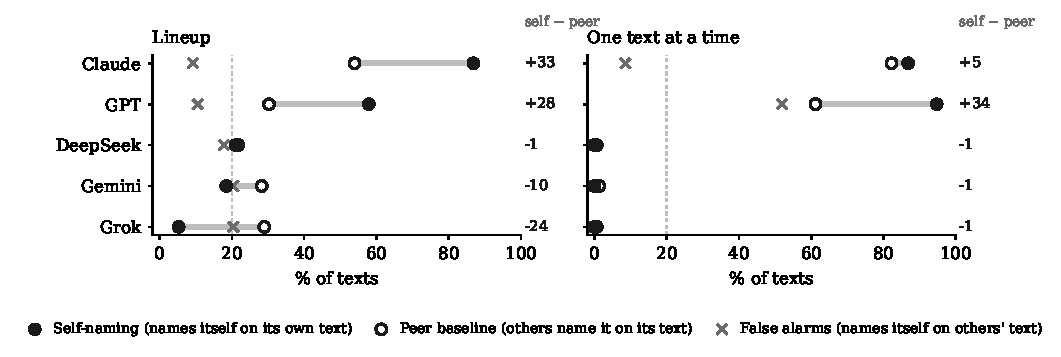
\includegraphics[width=\textwidth]{figures/lead.pdf}
  \caption{A self-naming rate (filled) means little on its own. Read it
  against the peer baseline (open: how often the other four judges name this
  judge on its text) and the false-alarm rate ($\times$: how often the judge
  names itself on text it did not write). Frontier panel, 38 texts per judge;
  the right-hand numbers are the self-advantage in points; dashed line, the
  20\% chance floor. In the lineup Claude and GPT beat their peers, Grok
  trails them. One text at a time, three judges never name themselves, and
  Claude's rate is matched by its peers.}
  \label{fig:lead}
\end{figure*}

Whether it can is usually measured with one number: how often a judge names
itself as the author of its own text, compared with chance. We argue that
this number, which we call the \emph{self-naming rate}, cannot answer the
question. A judge that names itself on 87\% of its own responses may
recognise its writing, or it may write text that \emph{anyone} can
attribute, or it may simply say ``me'' to everything. Separating the three
takes two more numbers from the same experiment (Figure~\ref{fig:lead}): how
often the judge names itself on text it did \emph{not} write (its
false-alarm rate), and how often the \emph{other} judges name it on its text
(its peer baseline). A judge recognises itself only if it beats that peer
baseline, a positive \emph{self-advantage}, and names itself more often on
its own text than on others', which we call \emph{discrimination}.

\begin{table}[t]
\centering\small
\setlength\tabcolsep{3pt}
\begin{tabular}{lll}
\toprule
Setting & Standard test & Our test \\
\midrule
Frontier, chat app, lineup & GPT, Claude & GPT, Claude \\
Frontier, chat app, single & GPT, Claude & GPT \\
Frontier, API, lineup & Claude, Grok & -- \\
Frontier, API, single & GPT, Claude & -- \\
Open-weight, lineup & Qwen & -- \\
Open-weight, single & Qwen, Llama, Phi & -- \\
Open-weight, yes/no & Llama, Mistral & -- \\
\midrule
Judge-settings flagged & 14 of 32 & 3 of 32 \\
\bottomrule
\end{tabular}
\caption{Which judges ``recognise themselves''. Standard test: the judge names itself on its own text more often than chance (Holm-corrected binomial test; for yes/no, says yes to its own text more than half the time). Our test: it beats its peers on its own text \emph{and} names itself more on its own text than on others' (both Holm-corrected permutation tests; for yes/no, AUC above 0.5). Nine judges, three corpora, three formats.}
\label{tab:verdicts}
\end{table}


We apply both tests to nine judges on three corpora. Five frontier models
(GPT-5.5, Claude Opus 4.7, Gemini 3.5 Flash, Grok 4.3 and DeepSeek)
attribute 190 texts they wrote in their chat apps for 38 prose prompts, and
600 texts they wrote through the API for 120 prompts in four genres
(argumentative prose, code, short answers and worked math). Four
open-weight models from four labs attribute \OWNResponses{} texts they wrote
for the same 120 prompts; their weights also let us read each judge's
likelihood of every text and rule out vendor watermarks. Judges name authors
in a lineup and one text at a time, and the open-weight judges also answer
``did you write this?'', in a fresh context or with their own answer to the
task in the conversation.

Three findings follow.
\begin{enumerate}
\item \textbf{The standard test is mostly wrong.} Of \SVPCells{}
judge--settings, the self-naming rate exceeds chance in \SVPStd{}; only
\SVPProper{} pass our test (Table~\ref{tab:verdicts}). The \SVPFalse{} false
positives (\SVPFalsePct{}) are judges that name themselves on much of what
they read: one text at a time GPT names itself on \FXGPTSingleNamesSelf{} of
all texts and Llama on \OWLlamaSingleNamesSelf{}, and asked ``did you write
this?'' Mistral says yes to \OWMistralBinaryFA{} of texts it did not write.
The standard test never missed a judge ours found.
\item \textbf{Real self-recognition is rare and does not travel.} Only Claude
and GPT pass, and only on the chat-app texts, where Claude's self-advantage
is \ClaudeAdvLineup{} points \ClaudeAdvLineupCI{} and GPT's \GPTAdvLineup{}.
On the 600 API texts no judge beats its peers, who name Claude's text almost
as readily as Claude does (\FXClaudeLineupPeer{} against
\FXClaudeLineupSelf{}). What holds across corpora is Claude's
discrimination: it names itself on \FXClaudeLineupSelf{} of its own texts and
\FXClaudeLineupFA{} of others'.
\item \textbf{Judges have the signal and do not use it.} A stylometric
classifier attributes the frontier texts at \EngineAAcc{} and the open-weight
texts at \OWClfPooled{}, and each open-weight judge's own likelihood picks
out its own text on \OWLikCondAccMin{} of prompts; yet what a judge claims as
its own does not follow its likelihood in any format, and none of the 1,900
reasons the frontier judges gave refers to the judge itself.
\end{enumerate}

The audit we propose needs no extra data, only the judgments a lineup
already produces (Section~\ref{sec:recs}): report a self-naming rate with its
false-alarm rate and peer baseline, test discrimination, never measure
recognition one text at a time, and measure each judge on the kind of text
it will judge. The stakes go beyond leaderboards: a monitor that reviews the
output of a copy of itself is only as independent as its inability to
recognise that output \citep{khullar2026selfattribution}.

% ===========================================================================
\section{Related work}
\label{sec:related}

\paragraph{Self-preference and self-recognition.}
LLM judges rate their own outputs above others'
\citep{panickssery2024selfpreference, wataoka2024perplexity, ye2025justice}.
\citet{panickssery2024selfpreference} tie the preference to self-recognition
through fine-tuning, and \citet{ackerman2025inspection} locate a
self-recognition direction in Llama-3-8B-Instruct.
\citet{wataoka2024perplexity} propose that the preference follows
familiarity: judges favour text of low perplexity to them, which their own
text usually is. Whether judges can \emph{name} their own text is less
settled. \citet{bai2025selfrecognition} find exact-author accuracy near chance
for ten models shown one text at a time, with guesses piling onto GPT and
Claude; \citet{davidson2024anonymized} find no consistent self-recognition in
anonymised panels; \citet{zhou2025implicit} find that models recognise their
own text in pairs but not alone; and \citet{laine2024sad} include
self-recognition in a situational-awareness benchmark.
\citet{stamand2026sgtr} show that a quality heuristic, picking the
better text as one's own, confounds many of these measurements, and
\citet{roytburg2026narcissists} and \citet{shi2025positionbias} document how
judge biases shift with format and position. Two studies are closest to
ours. CALM \citep{ye2025justice} scores self-enhancement against the scores
\emph{other} judges give the same answer, a peer reference for quality; we
apply the same idea to naming the author. \citet{barkhordar2026stylenotself}
show, for code, that raw attribution accuracy mostly reflects how readily a
model claims authorship and recommend balanced accuracy and heuristic
baselines. We reach the same diagnosis for prose and three other genres, and
add the peer baseline, the comparison of formats on identical texts, and
likelihood access for open-weight judges.

\paragraph{Where the self is located.}
\citet{khullar2026selfattribution} define \emph{self-attribution bias} as a
monitor rating an action more favourably when it is implicitly framed as its
own; the effect is strongest when the monitor judges an action it produced
earlier in the same conversation and largely vanishes for other models'
actions. That is a judgment shift driven by conversational position, not an
authorship decision, which is why we avoid the term and speak of self-naming.
Our on-policy condition (Section~\ref{sec:onpolicy}) connects the two: it
asks whether a judge that has just written an answer recognises it as its
own.

\paragraph{Attributing text to models.}
Supervised classifiers separate model families with high accuracy
\citep{sun2025stylometric, bitton2025fingerprints, rosenfeld2026whose,
zaitsu2025stylometry, russell2026storyscope}. \citet{sun2025stylometric}
report 97.1\% over five chat models and 88.9\% after shuffling the words of
every text, so much of the signal lies in the word distribution rather than
its order. Attribution systems also concentrate false attributions on some
candidates \citep{alipoormolabashi2025maui}, as LLM judges do on GPT and
Claude. Few-shot LLM judges can approach classifier accuracy
\citep{dietrich2026splits}; we study the zero-shot case, which is how
anonymised judging pipelines use them.

\paragraph{Watermarks.}
Keyed text watermarks bias token choice using a secret key and the preceding
context \citep{kirchenbauer2023watermark, dathathri2024synthid}; detecting
them requires the key. Google marks text from the Gemini app with
SynthID-Text \citep{dathathri2024synthid}, and Anthropic announced keyed
watermarking of Claude text in August 2026. Section~\ref{sec:watermark}
explains why neither can account for our results.

\paragraph{Explanations.}
Judges' stated reasons often omit the cues that actually drove their
decisions \citep{marioriyad2025silent}. We analyse the 1,900 rationales our
frontier judges wrote with that caveat (Section~\ref{sec:rationales}).

% ===========================================================================
\section{What a self-naming rate can and cannot show}
\label{sec:measure}

\paragraph{Terms.} A \emph{panel} is a set of models that both write the
texts and judge them, so that each judge has texts of its own among those it
judges. For judge $J$:
\begin{itemize}
\item the \textbf{self-naming rate} (hit rate) is the share of $J$'s own
texts that $J$ attributes to $J$;
\item the \textbf{false-alarm rate} is the share of texts $J$ did not write
that $J$ attributes to $J$;
\item the \textbf{peer baseline} is the share of $J$'s texts that the
\emph{other} judges attribute to $J$, i.e.\ how identifiable $J$'s writing is
to anyone else under the same protocol;
\item \textbf{self-advantage} is the self-naming rate minus the peer
baseline.
\end{itemize}
The first two are the hit and false-alarm rates of signal detection theory
\citep{green1966signal, macmillan2005detection}: they separate a judge's
ability to tell its own text from others' (sensitivity) from its readiness to
answer ``me'' (bias). The peer baseline adds what signal detection alone
does not: a reference for how attributable the text is. Self-advantage is
positive only if a judge does better on its own text than judges who did not
write it. It is not sufficient on its own: a judge that names itself on half
of everything it reads beats peers who rarely name it. A judge therefore
counts as self-recognising only if it also \emph{discriminates}, with a hit
rate above its false-alarm rate (tested by permuting which text in each
lineup is its own).

\paragraph{Three real cases.} All three come from our frontier panel
(Section~\ref{sec:frontier}). In the lineup, Claude names itself on 33 of its
38 texts (87\%), on only 14 of the 152 texts it did not write (9\%), and the
other four judges name Claude on 82 of their 152 judgments of Claude's texts
(54\%). It discriminates, and it beats its peers by 33 points: this is
self-recognition. Shown the same texts one at a time, Claude again names
itself on 33 of 38 with 13 false alarms, but now its peers name Claude on 125
of 152 (82\%), because in that format Claude receives over half of all
guesses, whoever wrote the text. The self-naming rate is unchanged; the evidence for
self-recognition is almost gone (+5 points). In the same format GPT names
itself on 36 of its 38 texts (95\%), which looks like the strongest
recognition in the study, but it also names itself on 79 of the 152 texts it
did not write (52\%): much of that rate is a readiness to say ``me''. The
self-naming rate alone cannot tell these three cases apart.

\paragraph{Which statistics we report.} For every judge and format we give
the self-naming rate with an exact 95\% interval, the false-alarm rate, the
peer baseline and the self-advantage with a prompt-level bootstrap interval.
Judgments on the same prompt are not independent (five judges see the same
five texts), so every test resamples or permutes whole prompts or whole
responses, never single judgments; Appendix~\ref{app:stats} gives the
effective sample sizes. For yes/no questions, which yield a probability of
``yes'' rather than a name, we report the area under the ROC curve (AUC) of
that probability for own versus others' texts, which is unaffected by a
judge's overall readiness to say yes.

% ===========================================================================
\section{Study 1: five frontier judges}
\label{sec:frontier}

\subsection{Design}
\paragraph{Corpus.} Five frontier models (GPT-5.5, Claude Opus 4.7, Gemini
3.5 Flash, Grok 4.3 and DeepSeek's chat model) each answered the same 39
argumentative prompts in their consumer chat apps at default settings,
between 15 June and 31 July 2026. Each prompt fixes the topic and the three
points the answer must make, and ends with a fixed instruction to write in
plain paragraphs with no lists, headers or bold, so the five answers to a
prompt say the same things and differ mainly in how they say them
(Appendix~\ref{app:corpus} has an example). Prompts come in three registers,
from everyday advice to philosophy. One prompt was dropped because two of its
five answers were corrupted copies, leaving 38 prompts and 190 responses.

\paragraph{Judges and formats.} The same five models judge, each through
OpenRouter at temperature~0, and each is the same model version that wrote
its share of the corpus, so ``self'' means the same model on both sides
\citep{panickssery2024selfpreference}.\footnote{Six of Claude's 38 texts were
written by Claude Sonnet 4.6 rather than Opus 4.7; dropping them leaves
Claude's lineup self-naming rate at 27/32 (84\%). The DeepSeek judge used the
provider's chat endpoint, whose snapshot we could record but not pin.}
Judges see only the responses, never the prompts. In the \emph{lineup}, a
judge sees all five responses to a prompt, labelled A to E, and names an
author for each; it is told that it may name the same model more than once.
Slot order follows a Latin square, so each author occupies each slot equally
often. In the \emph{single-text} format, a judge sees one response and names
its author from the same five. Each format yields 950 judgments. We parsed
all 1,900.

\paragraph{A fixed reference.} A random forest over 18 interpretable surface
features (length, punctuation and formatting rates, lexical diversity,
readability), trained and tested on disjoint prompts, attributes the same
responses at \EngineAAcc{} (95\% CI \EngineACI{}; chance \Chance{}). With
every length feature removed it still reaches \EngineALengthFreeLR{} with
logistic regression. The identifying signal is in the text. The comparison
with the judges is for zero-shot elicitation, without in-context examples or
access to likelihoods, which is how anonymised judging pipelines use a judge;
judges given labelled examples can approach classifier accuracy
\citep{dietrich2026splits}.

\subsection{Results}
\begin{table*}[t]
\centering\small\setlength\tabcolsep{3.5pt}
\begin{tabular}{llrrrrrr}
\toprule
Format & Judge & Self-naming & False alarms & Peer baseline & Self-adv. [95\% CI] & $p$ (Holm) & Skill-adj. \\
\midrule
Lineup & GPT & 22/38 & 16/152 & 46/152 & +27.6 [+10.5, +44.7] & $0.008$ & +19.3 \\
 & Claude & 33/38 & 14/152 & 82/152 & +32.9 [+21.1, +44.1] & $0.002$ & +35.1 \\
 & Gemini & 7/38 & 31/152 & 43/152 & $-$9.9 [$-$23.0, +4.6] & $0.619$ & $-$19.3 \\
 & Grok & 2/38 & 31/152 & 44/152 & $-$23.7 [$-$32.9, $-$13.2] & $0.008$ & $-$20.2 \\
 & DeepSeek & 8/38 & 27/152 & 33/152 & $-$0.7 [$-$15.1, +15.1] & $1.000$ & +11.4 \\
\midrule
Single & GPT & 36/38 & 79/152 & 93/152 & +33.6 [+25.0, +42.1] & $2.1\times10^{-4}$ & -- \\
 & Claude & 33/38 & 13/152 & 125/152 & +4.6 [$-$7.2, +14.5] & $1.000$ & -- \\
 & Gemini & 0/38 & 0/152 & 2/152 & $-$1.3 [$-$3.3, +0.0] & $1.000$ & -- \\
 & Grok & 0/38 & 0/152 & 1/152 & $-$0.7 [$-$2.0, +0.0] & $1.000$ & -- \\
 & DeepSeek & 0/38 & 0/152 & 1/152 & $-$0.7 [$-$2.0, +0.0] & $1.000$ & -- \\
\bottomrule
\end{tabular}
\caption{Study~1, frontier judges. Self-naming: the judge names itself on its own 38 texts. False alarms: it names itself on the 152 texts it did not write. Peer baseline: the other four judges name it on its texts. Self-advantage is the difference in rates, with a prompt-bootstrap interval; $p$ is the exact within-response randomisation test, Holm-corrected over the five judges. Skill-adjusted removes each judge's general accuracy and each author's identifiability (Appendix~\ref{app:stats}); it is not interpretable in single-text, where a judge's accuracy mostly reflects which model it habitually names. In single-text, Gemini, Grok and DeepSeek never name themselves.}
\label{tab:frontier}
\end{table*}


\paragraph{Two judges recognise themselves; one does the opposite.}
Table~\ref{tab:frontier} gives every quantity from
Section~\ref{sec:measure}. In the lineup, Claude's self-advantage is
\ClaudeAdvLineup{} points \ClaudeAdvLineupCI{} (randomisation
$p=$~\ClaudeAdvLineupP{}) and GPT's is \GPTAdvLineup{} \GPTAdvLineupCI{};
both keep false alarms near 10\%, so both also discriminate (hit minus
false-alarm rate \ClaudeDiscLineup{} and \GPTDiscLineup{} points,
within-lineup permutation $p$~\ClaudeDiscLineupHolm{}). DeepSeek (\DeepSeekAdvLineup{}) and Gemini
(\GeminiAdvLineup{}) show no advantage. Grok is significantly \emph{worse} on
its own text than its peers are (\GrokAdvLineup{} \GrokAdvLineupCI{}). The
verdicts for Claude, GPT and Grok survive Holm correction across judges and
every clustered test we ran (randomisation within responses, prompt
bootstrap, GEE, and a crossed random-effects model;
Appendix~\ref{app:stats}); so do the nulls for Gemini and DeepSeek, except
in the random-effects model, which absorbs judge skill (next paragraph). Clustering matters
little here: the four peer judgments on a response are nearly uncorrelated
(design effect \PeerDeffLineup{}).

\paragraph{Adjusting for judge skill.} A peer baseline built from strong
attributors is harder to beat than one built from weak ones. Removing each
judge's general accuracy and each author's general identifiability (an
additive difference-in-differences; Appendix~\ref{app:stats}) leaves Claude
at \ClaudeAdjAdvLineup{} \ClaudeAdjAdvLineupCI{}, GPT at \GPTAdjAdvLineup{}
\GPTAdjAdvLineupCI{} and Grok at \GrokAdjAdvLineup{}
\GrokAdjAdvLineupCI{}, and moves Gemini from neutral to
\GeminiAdjAdvLineup{} \GeminiAdjAdvLineupCI{}: Gemini is among the best
attributors of other models' text in the lineup but names itself on only 7 of
its own 38.

\paragraph{The format moves the rate, not the recognition.} One text at a
time, the judges send \SingleConcentration{} of all 950 guesses to GPT or
Claude, reproducing \citet{bai2025selfrecognition}. Gemini, Grok and DeepSeek
never name themselves, on their own text or anyone else's, so for them the
format measures nothing: their hit and false-alarm rates are both zero. GPT's
self-naming rate rises to \GPTSelfSingle{}, but so do its false alarms
(\GPTFALineupK{} to \GPTFASingleK{} of 152), and its signal-detection
sensitivity is unchanged between formats (log odds ratio 2.42 and 2.60,
$p=0.82$; Appendix~\ref{app:stats}). Claude keeps its self-naming rate
(\ClaudeSelfSingle{}) but loses its advantage (\ClaudeAdvSingle{}
\ClaudeAdvSingleCI{}), because its peers now name Claude on
\ClaudePeerSingleK{} of its 152 texts: in this format Claude receives
\ClaudeBlameSingle{} of all guesses whoever wrote the text. The peer baseline
is informative only where judges spread their guesses, which the lineup
forces and the single-text format does not.

\paragraph{Others' text.} Accuracy on text a judge did not write is above
the 20\% floor for most judge--format cells, but not all: Claude's lineup
cell (\ClaudeNonSelfLineupK{}/152, two-sided $p=$~\ClaudeNonSelfLineupP{})
and DeepSeek's lineup cell fail every clustered test. The ranking of judges
on others' text is a tie at the top in both formats (Appendix~\ref{app:stats}).

\subsection{At scale: 120 prompts, four genres}
\label{sec:frontier120}
\begin{table}[t]
\centering\small
\setlength\tabcolsep{2.5pt}
\resizebox{\columnwidth}{!}{%
\begin{tabular}{l rrr rr}
\toprule
Judge & Self & Peer & FA & Self-adv. [95\% CI] & Hit$-$FA \\
\midrule
GPT & 19.2\% & 15.0\% & 20.4\% & +4.2 [$-$3.3, +12.1] & $-$1.2 \\
Claude & 56.7\% & 50.4\% & 12.7\% & +6.2 [$-$2.5, +14.8] & +44.0$^{*}$ \\
Gemini & 26.7\% & 31.9\% & 18.3\% & $-$5.2 [$-$14.4, +3.8] & +8.3 \\
Grok & 32.5\% & 30.2\% & 16.2\% & +2.3 [$-$7.1, +11.9] & +16.2$^{*}$ \\
DeepSeek & 21.7\% & 18.8\% & 17.7\% & +2.9 [$-$5.2, +11.5] & +4.0 \\
\midrule
\multicolumn{6}{l}{\emph{One text at a time}} \\
GPT & 83.3\% & 63.1\% & 84.4\% & +20.2$^{*}$ [+13.5, +26.7] & $-$1.0 \\
Claude & 40.8\% & 49.8\% & 3.1\% & $-$9.0 [$-$16.0, $-$1.5] & +37.7$^{*}$ \\
Gemini & 8.3\% & 4.0\% & 4.8\% & +4.4 [$-$0.4, +9.6] & +3.5 \\
Grok & 1.7\% & 0.0\% & 0.6\% & +1.7 [+0.0, +4.2] & +1.0 \\
DeepSeek & 0.0\% & 10.6\% & 0.0\% & $-$10.6$^{*}$ [$-$12.9, $-$8.3] & +0.0 \\
\bottomrule
\end{tabular}}
\caption{Study~1 at scale: the five frontier judges on 600 texts the same five models wrote through the API for 120 prompts in four genres (120 own texts per judge). Columns as in Table~\ref{tab:frontier}; $^{*}$Holm-corrected within-prompt permutation $p<0.05$.}
\label{tab:frontier120}
\end{table}


Thirty-eight prose prompts is a small sample. We therefore had the same five
models answer all 120 prompts of Study~2, the 38 above among them, through
the API (temperature 0.7, no system prompt), and had the same five judges
attribute the 600 texts in the lineup (Table~\ref{tab:frontier120}).
\FXSingleSentence{}

\paragraph{No judge beats its peers at scale; Claude still discriminates.}
No self-advantage is significant on the 600 texts; the largest is Claude's,
\FXClaudeLineupAdv{} \FXClaudeLineupAdvCI{}. Claude names itself on
\FXClaudeLineupSelf{} of its own texts and on only \FXClaudeLineupFA{} of
others' (hit minus false-alarm rate \FXClaudeLineupDisc{} points, Holm
$p$~\FXClaudeLineupDiscHolm{}), but its peers now name Claude on
\FXClaudeLineupPeer{} of its texts. Grok, which trailed its peers on
chat-app prose, also discriminates (\FXGrokLineupDisc{}, Holm
$p=$~\FXGrokLineupDiscHolm{}); GPT, Gemini and DeepSeek do neither.

\paragraph{What changed.} Two things differ from Study~1, and the corpus
lets us separate them. On the 38 Study~1 prompts, re-collected through the
API, Claude's self-advantage is \FXOldClaudeLineupAdv{} and GPT's
\FXOldGPTLineupAdv{}: the same direction as in the chat-app corpus but
smaller, and neither survives Holm correction at this sample size, because
Claude's API prose is easier for its peers to name (\FXOldClaudeLineupPeer{}
against \ClaudePeerLineup{} for the chat-app texts). On the 82 new prompts and genres no
judge's self-advantage exceeds \FXNewLineupMaxAbsAdv{} points in either
direction, while Claude's discrimination holds (\FXNewClaudeLineupDisc{}).
Self-advantage moves with the texts; discrimination is the more stable
property.

% ===========================================================================
\section{Study 2: four open-weight judges, four genres}
\label{sec:openweight}

Study~1 has three limits: 38 prompts of one genre, closed models whose
probabilities we cannot read, and vendors that may mark their text. Study~2
removes all three.

\subsection{Design}
\paragraph{Panel.} Four open-weight instruction models from four labs:
Qwen2.5-7B (Alibaba), Llama-3.1-8B (Meta), Mistral-7B-v0.3 (Mistral AI) and
Phi-4-mini (Microsoft), each run in 4-bit on one consumer GPU
(Appendix~\ref{app:openweight}). With four candidates, chance is 25\%. As in Study~1, the same
weights write each model's share of the corpus and judge it.

\paragraph{Corpus.} 120 content-scaffolded prompts in four genres: the 40
argumentative prose prompts of the original bank and 20 new ones in the same
format; 20 Python functions with fully specified behaviour; 20 explanatory
questions answered in two to four sentences; and 20 word problems with a
numeric answer. Each model answered every prompt (temperature 0.7), giving
\OWNResponses{} texts\OnPolSecondSample{}. We generated the texts ourselves
from public weights, so none carries a watermark.

\paragraph{Conditions.} The \emph{lineup} and \emph{single-text} formats of
Study~1, with the panel's names as candidates. A \emph{yes/no} format asks a
judge of every text, in a fresh context, ``Did you write this text?''; we
read the probability of \emph{yes} from the judge's next-token distribution,
so every judge answers for itself on every text and both hit and false-alarm
rates are defined. \OnPolDesign{} Every judgment is greedy.
Finally, each judge's \emph{likelihood} of every text, conditioned on the
prompt, is read directly, and each judge rates every text in both corpora
for quality.

\subsection{Results}
\begin{table*}[t]
\centering\small
\setlength\tabcolsep{3.5pt}
\begin{tabular}{l rrrrr rrr rr}
\toprule
 & \multicolumn{5}{c}{Lineup} & \multicolumn{3}{c}{Yes/no, fresh context} & \multicolumn{2}{c}{Own likelihood} \\
\cmidrule(lr){2-6}\cmidrule(lr){7-9}\cmidrule(lr){10-11}
Judge & Self & Peer & FA & Self-adv. [95\% CI] & Hit$-$FA & Hit & FA & AUC & Pick-self & AUC \\
\midrule
Qwen & 56.7\% & 15.8\% & 49.2\% & +40.8$^{*}$ [+31.1, +50.6] & +7.5 & 51.7\% & 58.6\% & 0.45 & 100.0\% & 1.00 \\
Llama & 32.5\% & 22.2\% & 36.1\% & +10.3$^{*}$ [+1.9, +18.6] & $-$3.6 & 85.8\% & 85.6\% & 0.53 & 100.0\% & 1.00 \\
Mistral & 25.0\% & 20.8\% & 20.3\% & +4.2 [$-$6.1, +14.4] & +4.7 & 99.2\% & 99.4\% & 0.41$^{*}$ & 100.0\% & 1.00 \\
Phi & 20.8\% & 22.8\% & 22.5\% & $-$1.9 [$-$10.6, +6.9] & $-$1.7 & 4.2\% & 1.4\% & 0.53 & 100.0\% & 1.00 \\
\bottomrule
\end{tabular}
\caption{Study~2, open-weight judges, all four genres pooled (120 prompts). Lineup: self-naming, peer-baseline and false-alarm (FA) rates, the self-advantage with a prompt-bootstrap interval, and the hit minus false-alarm rate, which is positive only if a judge names itself more on its own text than on others'. Yes/no: ``Did you write this text?'' in a fresh context; hit and false-alarm rates at $P(\text{yes})>0.5$ and the AUC of $P(\text{yes})$ for own versus others' text (0.5 is chance). Own likelihood: the share of prompts on which the text the judge finds most likely, relative to the other judges, is its own (chance 25\%), and the AUC of that relative likelihood. $^{*}$Holm-corrected within-prompt permutation $p<0.05$ across the four judges.}
\label{tab:openweight}
\end{table*}


\paragraph{No open-weight judge recognises itself in the lineup.} Two
judges clear the first test of Section~\ref{sec:measure} and fail the
second (Table~\ref{tab:openweight}). Qwen names itself on
\OWQwenLineupSelf{} of its own texts while its peers name Qwen on only
\OWQwenLineupPeer{}, a self-advantage of \OWQwenLineupAdv{} points
\OWQwenLineupAdvCI{}; but it also names itself on \OWQwenLineupFA{} of the
texts it did not write, so its hits exceed its false alarms by only
\OWQwenLineupDisc{} points (Holm $p=$~\OWQwenLineupDiscHolm{}). Llama's
self-advantage of \OWLlamaLineupAdv{} \OWLlamaLineupAdvCI{} comes with
\emph{more} false alarms than hits (\OWLlamaLineupFA{} against
\OWLlamaLineupSelf{}). Both judges beat their peers on their own text only
because they put their own name on much of what they read. Mistral and Phi show neither
an advantage nor discrimination. The judges attribute the lineup at
\OWLineupAcc{} overall, against 25\% chance, although the texts carry the
signal: the classifier of Section~\ref{sec:frontier}, trained and tested on
disjoint prompts, attributes them at \OWClfPooled{} \OWClfPooledCI{}, from
\OWClfMath{} on math to \OWClfProse{} on prose.

\paragraph{One text at a time, each judge answers by habit.} The frontier
judges, shown one text at a time, piled their guesses onto GPT and Claude.
The open-weight judges pile them onto themselves, or onto no one: Qwen names
itself on \OWQwenSingleNamesSelf{} of all texts and Llama on
\OWLlamaSingleNamesSelf{}, whoever wrote them, while Mistral names itself on
only \OWMistralSingleNamesSelf{}. The self-advantage then measures the habit.
It is \OWQwenSingleAdv{} points for Qwen, \OWLlamaSingleAdv{} for Llama,
\OWPhiSingleAdv{} for Phi and \OWMistralSingleAdv{} for Mistral, all four
significant after Holm correction, and none of the four judges
discriminates (hit minus false-alarm rate \OWLlamaSingleDisc{} to
\OWPhiSingleDisc{} points, Holm $p\geq$~\OWPhiSingleDiscHolm{}). Read as
self-naming rates, this format would credit Qwen and Llama with near-perfect
self-recognition.

\paragraph{Asked directly, judges answer by disposition.} The yes/no format
removes the candidate list, so a judge cannot pile its answers onto one
popular name; it can only say yes or no to each text. What it says depends
almost entirely on the judge (Table~\ref{tab:openweight}). Mistral says yes
to \OWMistralBinaryHit{} of its own texts and to \OWMistralBinaryFA{} of
everyone else's; Llama to \OWLlamaBinaryHit{} and \OWLlamaBinaryFA{}; Qwen
to \OWQwenBinaryHit{} and \OWQwenBinaryFA{}; Phi to \OWPhiBinaryHit{} and
\OWPhiBinaryFA{}. Read as self-naming rates, these would rank the four judges
from near-certain self-recognition to none; read against the false alarms,
none of them discriminates. The AUC of $P(\text{yes})$, which is free of that
disposition, is \OWQwenBinaryAUC{} for Qwen, \OWLlamaBinaryAUC{} for Llama,
\OWPhiBinaryAUC{} for Phi and \OWMistralBinaryAUC{} \OWMistralBinaryAUCCI{}
for Mistral, which is reliably \emph{below} chance (within-prompt
permutation, Holm $p=$~\OWMistralBinaryAUCHolm{}): Mistral is slightly more
willing to claim other models' text than its own. Split by genre, the
highest AUC of any judge is \OWBinaryAUCGenreMax{} \OWBinaryAUCGenreMaxCI{}
(\OWBinaryAUCGenreMaxWho{}).

\subsection{On-policy judging}
\label{sec:onpolicy}
\citet{khullar2026selfattribution} find that a monitor's judgment shifts
most when it evaluates an action it produced earlier in the same
conversation. Our on-policy conditions ask whether that position also lets a
judge recognise its writing. When the candidate is the judge's own previous
turn, word for word, every judge's $P(\text{yes})$ separates it from peers'
answers: the AUC is \OWMistralOnPolAUC{} for Mistral, \OWQwenOnPolAUC{} for
Qwen, \OWPhiOnPolAUC{} for Phi and \OWLlamaOnPolAUC{} for Llama (all Holm
$p<0.01$). That is a low bar, since the candidate is a copy of text already in
the context window, and even so it is not met everywhere: on prose Llama's
AUC is \OWLlamaOnPolProseAUC{}, below chance, and its thresholded answers keep
the habits of the fresh-context format (Mistral says yes to
\OWMistralOnPolFA{} of peers' answers). \OnPolResampled{}

% ===========================================================================
\section{What the judges use}
\label{sec:mechanism}

The classifier shows that the frontier texts carry enough signal to name
their authors at \EngineAAcc{}. The frontier judges reach at most
\GPTOverallLineup{} overall. We test four accounts of what they use instead.

\subsection{Rationales}
\label{sec:rationales}
Every frontier judgment came with a one-sentence reason. We coded all 1,900
with a transparent rule-based scheme of eleven cue types (length,
punctuation and formatting, structure, sentence construction, word choice,
tone, hedging, rhetorical flourish, appeals to a model's typical style,
references to the judge itself, and content). \RationaleValidation{}

\emph{No judge ever refers to itself.} Not one of the 1,900 reasons says
anything like ``this is how I write'', including the 66 in which Claude
correctly named itself. Judges instead appeal to what a model typically
writes: 46\% of lineup reasons and 95\% of single-text reasons invoke a
model's characteristic style (``classic Claude hedging'').

\emph{The cited cues are the same whether a self-naming is right or wrong.}
When Claude names itself on its own text in the single-text format it cites
hedging 31 times in 33; when it names itself on a text it did not write, 12
times in 13. GPT's self-namings cite word choice in 33 of 36 hits and 64 of
79 false alarms. A judge that recognised its own writing would not describe
its misses in the same terms as its hits; a judge applying a stereotype of
itself would.

\emph{The cues are mostly true of the text, but not diagnostic.} When a
lineup reason calls a response long, that response is the longest of the
five in 47 of 71 cases (chance 20\%), and phrases judges quote appear
verbatim in 238 of 245 cases. The exception is ``sophisticated vocabulary'',
which matches the response with the longest words no more often than chance
(3 of 35). Judges describe the texts accurately and then map the description
onto a model by reputation. Citing hedging predicts a correct attribution
(odds ratio 1.96, $p<10^{-4}$, lineup), but that shrinks once the true
author is controlled for (1.54, $p=0.017$), because hedging is simply common
in Claude's text. As \citet{marioriyad2025silent} warn, none of this shows
what drove a decision; it shows what judges say drove it.

\subsection{Generative match}
\label{sec:genmatch}
\citet{wataoka2024perplexity} propose that a judge favours, and perhaps
claims, text it would itself have produced. With closed models we can
approximate ``what $J$ would write'' by $J$'s own answer to the same prompt,
and ask whether a text's similarity to it predicts $J$ naming itself on text
it did not write. It does not: across three similarity measures (stylometric
distance, word and character $n$-gram cosine, function-word profile), two
formats and five judges, 1 of 36 clustered models reaches $p<0.05$. GPT, the
judge with the most such false alarms (79 in single-text), shows odds ratio
1.52 [0.85, 2.71] per standard deviation of stylometric similarity. Nor do
judges name the model whose answer to the prompt is most similar to the
text: in 630 wrong lineup attributions the named model is the most similar
one 31.9\% of the time against 30.1\% for shuffled guesses ($p=0.12$),
although the same similarity measures identify the true author 74--79\% of
the time. The signal a generative-match strategy would need is present; the
judges' errors do not follow it. Section~\ref{sec:likelihood} tests the
account directly, with each open-weight judge's own probabilities.

\subsection{Likelihood}
\label{sec:likelihood}
\citet{wataoka2024perplexity} tie self-preference to familiarity: a judge
favours text that is likely under its own distribution, which its own text
usually is. Open weights let us read that familiarity directly. For every
judge and every text we compute the mean token log-probability of the text
as the judge's reply to its prompt, and subtract the mean of the other three
judges' values for the same text, so that a text predictable to every model
does not count as familiar to one.

\emph{Each judge's probabilities identify its own text.} Picking, for each
prompt, the text a judge finds relatively most likely names its own text on
\OWLikCondAccMin{} of prompts for every judge (chance 25\%), and on \OWLikUncAccMin{}--\OWLikUncAccMax{} even without the
prompt. This is expected, since each text was sampled from its author, but
it means that the information needed to recognise one's own text is present
in every judge's forward pass.

\emph{The judges' answers do not use it.} If familiarity drove self-naming,
a judge would claim the texts of others that it finds relatively likely more
often than those it does not. We test this within each prompt, on texts the
judge did not write, comparing the standardised relative likelihood of the
texts it named as its own with the rest (within-prompt permutation). Across
the \OWFamTests{} judge--format pairs with enough claims to test (lineup,
single text and yes/no; \OWFamUntestable{} pairs claim everything or nearly
nothing), none survives Holm correction; the smallest $p$ is
\OWFamMinP{} (\OWFamMinWho{}; Holm \OWFamMinHolm{}), and there the judge
claims the texts it finds \emph{less} likely. Asked who wrote a text, a judge
answers without consulting the one signal that would let it know.

\subsection{Quality}
\label{sec:quality}
\citet{stamand2026sgtr} show that a judge can appear to recognise itself by
claiming whichever text it rates best. Each open-weight judge rated every
text in both corpora for how well it carries out its task, on a 1--9 scale
read as the expected value over the judge's probabilities for the nine
digits.

\emph{Frontier self-naming is not a quality effect.} With the four
open-weight judges as raters independent of the frontier judges, we ask two
questions of Study~1. Do frontier judges claim the better texts? Among texts
a judge did not write, the ones it named as its own are rated no higher than
the rest for any judge in the lineup (within-prompt permutation, smallest
$p=$~\QFLineupClaimMinP{}, Gemini, whose claims lean towards worse texts);
one text at a time, GPT, the one judge that often claims others' text,
claims the \emph{worse} ones (standardised difference \QFGPTSingleClaimDiff{},
$p=$~\QFGPTSingleClaimP{}). Does self-advantage survive holding quality
fixed? In a GEE of correctness on whether the judge wrote the text and the
text's within-prompt quality, the self term stays significant for Claude
(odds ratio \QFClaudeLineupOR{}, $p=$~\QFClaudeLineupORP{}), GPT
(\QFGPTLineupOR{}, $p=$~\QFGPTLineupORP{}) and Grok (\QFGrokLineupOR{},
$p=$~\QFGrokLineupORP{}). The raters agree only weakly (mean pairwise
Spearman \QFRaterRho{}), since almost every frontier text is rated near the
top of the scale (author means \QFMeanLo{}--\QFMeanHi{}), so this measures
quality coarsely.

\emph{The open-weight judges do not prefer their own text either.} We
measure self-preference as how much more a judge rates its own text than its
peers rate it, minus how much more it rates others' text than its peers do,
so that a generous rater is not counted as self-preferring. It ranges from
\OWQualSelfPrefMin{} to \OWQualSelfPrefMax{} points on the nine-point scale,
and every prompt-bootstrap interval includes zero (largest: Mistral,
\OWMistralQualSelfPref{} \OWMistralQualSelfPrefCI{}). Judges that cannot tell
their text from others' do not favour it.

% ===========================================================================
\subsection{Not a watermark}
\label{sec:watermark}

Could a judge be reading a watermark its vendor planted? Three facts say no.

\emph{A keyed watermark cannot be read in context.} Deployed text watermarks
shift token probabilities by a pseudorandom function of a secret key and the
preceding tokens \citep{kirchenbauer2023watermark, dathathri2024synthid}.
Detection needs the key; the pattern is statistically invisible without it,
by design. Nothing in our protocol gives a judge a detector.

\emph{The dates do not fit.} Our frontier corpus was written between 15 June
and 31 July 2026. Anthropic announced keyed watermarking of Claude text in
August 2026, applied at launch to models released from 2 August and
retrofitted to older models, Opus 4.7 among them, without a stated start date
\citep{anthropic2026watermark, anthropic2026marking}. The judge with the
largest self-advantage wrote its texts before any announced Claude watermark.
Conversely, text from the Gemini app is watermarked with SynthID-Text
\citep{deepmind2026synthid}, and Gemini is one of the judges that does
\emph{not} recognise itself.

\emph{Authorship is identifiable without one.} We generated the open-weight
corpus ourselves from public weights, with no sampling modification, so it
carries no watermark; the stylometric classifier still attributes it at
\OWClfPooled{} (Section~\ref{sec:openweight}). The signal that would let a
judge recognise its own text is stylistic and needs no watermark, and the
open-weight judges, which could not be reading one, do not recognise
themselves either.


% ===========================================================================
\section{Recommendations}
\label{sec:recs}

\begin{enumerate}
\item \textbf{Report three numbers and test two things.} A self-naming rate
is uninterpretable without the false-alarm rate and the peer baseline; claim
recognition only if the judge beats its peers and discriminates, with tests
that respect the clustering of judgments within prompts.
\item \textbf{Do not measure recognition one text at a time.} In that format
judges collapse onto one or two names; three of our five frontier judges
never named themselves at all, so their recognition was unmeasurable, and
the peer baseline was inflated for the model everyone guessed. Use a lineup,
or a yes/no question scored by its ROC curve.
\item \textbf{Treat leakage as a property of each judge and each text
distribution.} Whether a judge can spot its own outputs varied from strongly
positive to significantly negative within one panel, and the same judges'
self-advantages shrank to nothing on a larger corpus collected differently.
Anonymisation protects a pipeline only against the judges that cannot
recognise themselves on the texts it actually judges; measure each judge on
such texts before relying on it, and do not assume a mixed panel averages the
risk away.
\item \textbf{Do not read mechanism off rationales.} Judges' stated reasons
describe the text accurately but cite the same cues when a self-naming is
wrong as when it is right (Section~\ref{sec:rationales}): they show what a
judge associates with a model, not how it decided.
\end{enumerate}

% ===========================================================================
\section{Limitations}
\label{sec:limits}

\paragraph{Scale.} Study~1's chat-app corpus has 38 prompts per judge, so a
single judge's self-naming rate there rests on 38 judgments and intervals are
wide (Table~\ref{tab:frontier}); its verdicts for Claude and GPT did not
reach significance on the 120-prompt API corpus (Section~\ref{sec:frontier120}). Study~2 has \OWNPrompts{} prompts but uses
4--8B-parameter judges run in 4-bit, which are weaker attributors than
frontier models; its results show what open-weight judges of that size do,
not what larger ones would.

\paragraph{Genres.} Study~1 is argumentative prose only. Study~2 adds code,
short answers and worked math, but every prompt is content-scaffolded and in
English; dialogue, long documents and other languages are untested.

\paragraph{Corpus provenance.} The frontier corpus was collected by hand in
consumer chat apps, whose hidden system prompts and default decoding we
cannot observe; six of Claude's 38 texts came from Claude Sonnet 4.6, and
the DeepSeek text and judge could be matched by name but not pinned to one
snapshot. Judge calls went through OpenRouter, which routed DeepSeek across
three hosts (accuracy did not differ by host, $\chi^2=2.01$, $p=0.37$). The
120-prompt corpus was collected through the API instead, with no system
prompt and at temperature 0.7, on 1 October 2026, two to three months after
the chat-app corpus, and
through the same unpinned DeepSeek endpoint, which wrote and judged within
the same hour; the two corpora differ in channel as well as in size, and
Section~\ref{sec:frontier120} separates the two only as far as the 38 shared
prompts allow.
Study~2's models ran as NF4 checkpoints re-packed to 4-bit groups of 32
(Appendix~\ref{app:openweight}); the same weights wrote and judged, so
``self'' is exact, but they are not the labs' bf16 releases.

\paragraph{What judges saw.} Judges never saw the prompt, except in the
on-policy conditions, which give a judge the task and its own answer.

\paragraph{Quality.} Judges may name themselves on the texts they rate best
\citep{stamand2026sgtr}. We measure quality with an independent panel and
control for it (Section~\ref{sec:quality}), but a rater panel is itself a
set of judges with their own preferences, and ours rated almost every
frontier text near the top of the scale, so quality is controlled only
coarsely.

\paragraph{Formats per panel.} The yes/no, on-policy and quality
conditions, and the likelihood analysis, were run on the open-weight panel
only. For the frontier judges we have the lineup and single-text formats on
the two frontier corpora; whether they behave like the open-weight judges in
the other formats is untested.

% ===========================================================================
\section{Conclusion}
\label{sec:conclusion}

A judge that names itself as the author of its own text is not thereby
recognising itself. Scored against its false alarms and against what its
peers achieve on the same text, frontier judges' self-recognition on
chat-app prose was confined to two of five, absent in two and reversed in
one; on a larger corpus of API text in four genres, the advantage over peers
disappeared and only Claude's ability to tell its own text from others'
remained. A single-text protocol hides all of this behind whichever names
the judges favour. Four open-weight judges, whose own probabilities single
out their own text, recognise it only with their own answer to the task in
view, and then not all of them; two would pass for strong self-recognisers to
anyone reading only a self-naming rate. The practical consequence is that
the risk of a judge spotting, and favouring, its own outputs has to be
measured judge by judge, on the kind of text the pipeline judges and with a
peer baseline, before anonymisation can be trusted to remove it.


\bibliography{references}
\bibliographystyle{acl_natbib}

\appendix
% ===========================================================================
% Appendices: replication details (TACL category 1, up to 5 pages) and
% complementary tables (category 2, up to 3 pages). Not reviewed; every
% load-bearing result is in the body.

\section{Corpus and protocol}
\label{app:corpus}

\paragraph{Release.} Both corpora, all judgments with their confidence
ratings and reasons, every archived API response, the prompts and the
analysis code will be released with the paper; every number in it is
regenerated from them by one script.

\paragraph{Example prompt (E1, verbatim).}
\emph{Argue that getting enough sleep each night improves how well you
function the next day. Cover three specific effects: sharper focus and
memory, better mood and emotional control, and improved physical energy.
Write in continuous prose paragraphs only. Do not use bullet points,
numbered lists, headers, bold text, or any other formatting.}

\paragraph{Frontier corpus.} 39 prompts in three registers (13 each),
answered by each model in its consumer chat app, in a fresh conversation,
with memory and custom instructions off, between 15 June and 31 July 2026.
Prompt M5 is excluded: its DeepSeek answer is a verbatim copy of its Grok
answer and its Gemini answer a copy of another prompt's. H3's DeepSeek answer
is truncated (266 words) and kept. Mean length runs from 324 words (Grok) to
689 (DeepSeek).

\paragraph{Judge requests.} OpenRouter, temperature 0, 8,000 output tokens
(16,000 for Gemini, whose reasoning tokens count against the limit), 16--17
August 2026. Slugs: \texttt{openai/gpt-5.5},
\texttt{anthropic/claude-opus-4.7}, \texttt{google/gemini-3.5-flash},
\texttt{x-ai/grok-4.3}, \texttt{deepseek/deepseek-chat}. Of 1,140 calls,
Claude was served by Anthropic on 227 and Google on 1; DeepSeek by three
hosts. The lineup and single-text instructions are reproduced in the
released code.

\section{Statistical details}
\label{app:stats}

\paragraph{Randomisation test for self-advantage.} For judge $J$, each of
$J$'s 38 texts was judged once by each of the five judges. Under the null
that the author's own judgment is no more likely to be correct than a
peer's, the five judgments on a text are exchangeable with respect to which
judge is labelled ``self''. Relabelling one of the five uniformly at random,
independently per text, gives a Poisson-binomial null for the self-advantage
statistic, from which we compute exact two-sided $p$-values. Because each
text's number of correct judgments is held fixed, the test conditions on how
identifiable each text is, and it keeps a text's four peer judgments
together, which Fisher's exact test does not.

\paragraph{Other clustered analyses.} Prompt-level bootstrap (10,000
resamples) for every interval on a rate built from 152 judgments; GEE
logistic regression of correctness on a self indicator with an exchangeable
working correlation within prompt and a bias-reduced sandwich estimator;
and a crossed random-effects logistic model with random intercepts for prompt
and judge. Holm correction is applied within each family: the five
self-advantage tests per format, the five self-rate-versus-chance tests per
format, and the ten non-self-versus-chance tests. After correction, Grok's
lineup self-naming rate is no longer significantly \emph{below} chance
(Holm $p=$~\GrokSelfLineupHolm{}), though its negative self-advantage is.

\paragraph{Effective sample size.} The intraclass correlation of correctness
among the four peer judgments of a text is 0.014 in the lineup (design effect
\PeerDeffLineup{}, about \PeerNeffLineup{} effective judgments of 152).

\paragraph{Skill adjustment.} The additive adjustment compares $J$'s
advantage on its own text with the advantage each peer $K$ shows over the
remaining judges on third-party text, i.e.\ a difference in differences that
removes general judge skill and general author identifiability. A ratio
version and a GEE model with judge and author fixed effects agree in sign
for every lineup judge.

\paragraph{Signal detection.} We summarise a judge's $2\times2$ table of hits
and false alarms by a Haldane-corrected log odds ratio. When a judge never
names itself (a row of the table is empty) the statistic is undefined, which
is the case for three of five judges in the single-text format.

\section{Open-weight panel}
\label{app:openweight}

\paragraph{Models.} Qwen2.5-7B-Instruct (Alibaba), Llama-3.1-8B-Instruct
(Meta), Mistral-7B-Instruct-v0.3 (Mistral AI) and Phi-4-mini-instruct
(Microsoft), each from Unsloth's NF4 export on the Hugging Face Hub.
Gemma-2-9B-it (Google) was planned as a fifth judge and dropped before any
judging: with its 256k-entry vocabulary it did not fit in the memory of our
one machine (an 8\,GB laptop GPU sharing 32\,GB of RAM), and no result was
computed with it.

\paragraph{Quantisation.} We dequantise each NF4 layer and re-pack it as asymmetric
4-bit integers in groups of 32 for PyTorch's built-in 4-bit matrix kernel,
on one 8\,GB laptop GPU; embeddings, norms and output layers stay in
bfloat16. The re-pack adds about 8\% relative rounding error per layer and
shifts mean token log-probabilities by about 0.1 nats against exact NF4
inference; the same weights write each model's corpus and serve as its
judge, so this does not affect which text is a judge's own.

\paragraph{Decoding.} Corpus: temperature 0.7, top-$p$ 0.95, fixed seeds,
up to 1,100 new tokens for prose, 900 for code and math, 300 for short
answers; two independent samples per prompt. Judging: greedy decoding for the
lineup and single-text formats; for yes/no and quality questions we read the
next-token probabilities of the answer options directly and report the
probability mass they hold, which checks that the judge answered in format.
An option's probability is that of the first token carrying it under each of
its spellings (``Yes'', `` yes'', \ldots), skipping tokens that are only
whitespace, since all four tokenizers split `` 7'' into a space token and
``7''. Where a judge's most likely next token is itself bare whitespace
(Mistral's ratings, never a yes/no answer), we append it and read the
options one position later. The options held at least 89\% of the
probability in every yes/no judgment. In ratings, Qwen, Llama and Mistral put
all of it on the nine digits; Phi put a median of 81\% there for the
open-weight texts (minimum 12\%) and 94\% for the frontier texts, so its
ratings, renormalised over the digits, are the least reliable of the four. Prompts longer than 512 tokens are pre-filled in 512-token chunks
through the key--value cache, which changes memory use and nothing else
beyond floating-point rounding.

\paragraph{Consistency of each model's style.} A second, independent
sample from each model for every prompt lets us ask whether a model's style
is a property of the model or of one draw. The classifier of
Section~\ref{sec:openweight}, trained on the first sample of the training
prompts and tested on the second sample of the held-out prompts, attributes
\OWClfCrossSample{} \OWClfCrossSampleCI{} of texts, against \OWClfPooled{}
within the first sample: the signal the judges fail to use is stable across
samples.

\begin{table}[t]
\centering\small
\setlength\tabcolsep{3pt}
\resizebox{\columnwidth}{!}{%
\begin{tabular}{ll rr rrr}
\toprule
 & & \multicolumn{2}{c}{Lineup} & \multicolumn{3}{c}{Yes/no AUC} \\
\cmidrule(lr){3-4}\cmidrule(lr){5-7}
Genre & Judge & Self-adv. & Hit$-$FA & Fresh & On-pol. & Resamp. \\
\midrule
Prose & Qwen & +58.9 & +8.3 & 0.47 & 0.86 & 0.60 \\
 & Llama & +10.6 & $-$3.9 & 0.51 & 0.30 & 0.28 \\
 & Mistral & +5.0 & +5.0 & 0.37 & 0.89 & 0.45 \\
 & Phi & +6.7 & $-$1.7 & 0.56 & 0.76 & 0.69 \\
\midrule
Code & Qwen & +10.0 & +6.7 & 0.48 & 0.99 & 0.76 \\
 & Llama & +6.7 & $-$11.7 & 0.64 & 1.00 & 0.71 \\
 & Mistral & +8.3 & +16.7 & 0.52 & 0.99 & 0.52 \\
 & Phi & $-$13.3 & $-$8.3 & 0.50 & 0.89 & 0.65 \\
\midrule
Short & Qwen & +15.0 & +1.7 & 0.29 & 0.98 & 0.82 \\
 & Llama & +23.3 & +11.7 & 0.51 & 0.93 & 0.43 \\
 & Mistral & +3.3 & +0.0 & 0.40 & 0.98 & 0.36 \\
 & Phi & $-$5.0 & $-$5.0 & 0.41 & 0.84 & 0.50 \\
\midrule
Math & Qwen & +43.3 & +11.7 & 0.53 & 0.79 & 0.70 \\
 & Llama & +0.0 & $-$10.0 & 0.50 & 0.33 & 0.37 \\
 & Mistral & $-$1.7 & $-$3.3 & 0.42 & 0.82 & 0.34 \\
 & Phi & $-$13.3 & +8.3 & 0.58 & 0.55 & 0.61 \\
\bottomrule
\end{tabular}}
\caption{Study~2 by genre (per judge: 60 lineups and 240 yes/no judgments for prose, 20 and 80 for each other genre). Lineup: self-advantage and hit minus false-alarm rate, in points. Yes/no: AUC of $P(\text{yes})$ for own versus others' text in a fresh context, with the judge's own answer verbatim in the conversation (on-policy), and with a second sample of its own as its turn (resampled); 0.5 is chance.}
\label{tab:genre}
\end{table}


\paragraph{Prompts.} 120: the 40 prompts of the original bank, 20 new prose
prompts in the same scaffold, 20 Python functions with fully specified
behaviour, 20 short explanatory questions answered in two to four sentences,
and 20 word problems with a unique numeric answer. All are released.

\section{Rationale coding}
\label{app:rationales}

\paragraph{Scheme.} Eleven multi-label cue categories assigned by regular
expressions over the one-sentence reason attached to every judgment; the
lexicon and codebook are released. A reason matching none is coded
\emph{other} (none of the 1,900 was).

\paragraph{Validation.} 150 reasons stratified by judge and format (100 used
to revise the lexicon once, 50 held out) were labelled from the reason text
alone. The first annotator, an instance of an LLM (Claude) that also wrote
the lexicon, gives holdout micro precision 93.1\% and recall 99.5\%. A
second, independent instance that saw only the codebook agreed with the
rules at 97.0\% precision and 95.7\% recall over all 150 (per-category
$\kappa$ 0.86--1.00). Claude is also one of the judges, so biases shared by
annotator and judge cannot be ruled out by these two. \RationaleHumanAppendix{}

\paragraph{Faithfulness checks.} For cues with a measurable counterpart we
compared the cited property with the five responses to the same prompt:
``long'' against word count, ``long sentences'' against mean sentence
length, quoted phrases against the text, and ``sophisticated vocabulary''
against mean word length.


\end{document}
